\chapter{Exact Algorithm}
\label{sec:exact_algo}

\section{Overview}
\label{subsec:exact_algo_overview}

\begin{observation}
	\label{ob:frequency}
	If two subgraphs have higher support values individually, it is very likely
	that the pair will also have a higher correlation.
\end{observation}

\begin{observation}
	\label{ob:dfs}
	For highly (e.g., top-$k$) correlated subgraphs mining, generally a
	breadth-first or a best-first exploration of the search space is more
	efficient compared to a depth-first traversal of the search space.
\end{observation}

Setting $k$ to infinity would enable us to mine all pairs of correlated subgraph
patterns. However, on the contrary, it is hard to control the value of {\sf
Min-sup} to get the result of a particular $k$ of {\sf Top-$k$} correlated
subgraphs. That is to say, the {\sf Min-Sup} problem can be transfered from {\sf
Top-$k$} problem. As a result, we concentrate on {\sf Top-$k$} problem in the
following sections.

% \setlength{\parskip}{0.3em}
\spara{\raggedleft \textbf{Pattern Search Tree.}} All operations including
correlation computation and subgraph pattern extension are performed on patterns
following an order on a \textit{pattern search tree}. We denote this tree as
$T$. Each node $Q\in T$ represents a subgraph pattern. We denote the set of
current \textit{leaf} nodes in $T$ as $Leaf(T)$. Each element $Q_l\in Leaf(T)$
is a pattern that has not yet been $operated$ for correlation computation. A
node $Q_l\in Leaf(T)$, once operated, is inserted into the $operated$ set.
% \setlength{\parskip}{0em}

% \subsection{Order of Subgraph Generation and Correlation Calculation}

\par The correlated subgraph mining algorithm is an iterative procedure,
essentially consisting of the following steps: \par 1) select a node $Q_i$ from
$Leaf(T)$, i.e. $Q_i\in Leaf(T)$, and pop out $Q_i$ from $Leaf(T)$, i.e.
$Leaf(T)=Leaf(T)\setminus Q_i$. \par 2) calculate $\tau(Q_i,Q_j,h)$, for all
$Q_j\in operated$ \par 3) try to extend $Q_i$ to $Ex(Q_i)$, where $Ex(Q_i)$ is
the set of all the possible subgraphs extended from $Q_i$. \par 4) Check the
frequency of $Q_i',Q_i'\in Ex(Q_i)$ based on MNI support, $\sigma(Q')$, if
$\sigma(Q_i')\ge$ {\sf Min-Sup}. we put $Q_i'$ into $Leaf(T)$.
\begin{thrm}
	The order of subgraph generation and correlation calculation will not miss
	any correlated pairs between any of two frequent subgraphs.
\end{thrm}
% After step 4, we give $Q_i'$ an index of frequent subgraph discovery order,
% denoted as $index(Q_i')=a$, which means $Q_i'$ is the $a$-th subgraph in $T$.
% After the loop, we give $Q_i$ an index of correlation calculation order,
% denoted as $corIndex(Q_i)=b$, which means $Q_i$ is the $b$-th subgraph in $T$
% which and we put $Q_i$ into $Cor(T)$, i.e. $Cor(T)=Cor(T)\cap Q_i$.

\subsection{Best-first Exploration}
\label{subsubsec:exact_algo_bestfs}
Observation \ref{ob:frequency} suggests that faster convergence of the algorithm
could be expected if a subgraph pattern having a higher support is
\textit{operated} preceding every other pattern in $Leaf(T)$. As a result, we
use a naive rule to determine the priority of the leaf nodes in $Leaf(T)$: $Q_1$
has a higher priority than $Q_2$ \forall $Q_1, Q_2 \in Leaf(T)$ if and only if:
\begin{align*}\sigma(Q_1)>\sigma(Q_2)\end{align*}
Utilizing the estimating rule above, if the current leaf node $Q_k$ in the search tree has a highest support among all the other elements in the set of the leaf nodes, i.e. $\sigma(Q_k)=\max\{\sigma(Q_i)|Q_i\in Leaf(T)\}$. Then, $Q_k$ has the priorty to be calculated and extended.


\subsection{Termination Criteria}
\label{subsubsec:exact_algo_ceasing}
Obviously, our purpose is to find $k$ pairs of correlated subgraphs and guarantee that the other pair of subgraphs could not have a higher correlation $\tau$. Retrospect the properties mentioned in Section \ref{sec:overview}, assume $Q$ is a frequent subgraph of the data graph, $Q_k$ is an arbitary frequent subgraph of the data graph. We denote $Sup(Q)$ as the set of all the possible supergraphs of $Q$ and $Q'\in Sup(Q)$. Then, the following condition always holds:
\begin{align*} \tau(Q',Q_k,h)\le \sigma(Q') \end{align*}
\begin{align*} \sigma(Q')\le \sigma(Q) \end{align*}
It is easy to get following upperbound of $\tau(Q',Q_k,h)$ by combining the two conditions above:
\begin{align*} \tau(Q',Q_k,h) \le \sigma(Q) \end{align*}
Consider this upperbound, if $\sigma(Q)$ does not reach the minimum number of
being a candidate of {\sf Top-$k$} set, i.e. $\sigma(Q)<\tau(Q_i,Q_j,h)$ for all
the $i, j$ in the current {\sf Top-$k$} set, then all the correlations
containing $Q$, $\tau(Q,Q_k,h)$, as well as all the correlations containing
$Q'$, $\tau(Q',Q_k,h)$, are impossible to be the elements in {\sf Top-$k$} set.
\par On the other hand, we have to consider another possible circumstance, where
there are no $k$ correlated pairs in this graph at all. In that case, the number
of elements in {\sf Top-$k$} set has not reached $k$ but all the support value
of the leaf nodes are already below the minimum support. As a consequence, this
condition is also a signal telling us to stop the search. \par Formally, we fix
the condition of not adding $Q$ to $Leaf(T)$, which is, suppose $|Topk|$ is the
number of elements in {\sf Top-$k$} set, $min\_sup$ is the minimum support of
the correlation, we stop our search if either both of the following conditions
holds.
\begin{align*} \sigma(Q)\le min\{t|t\in Top\_k\}\end{align*}
\begin{align*} |Top\_k|=k \end{align*}
or following condition holds.
\begin{align*} \sigma(Q)\le min\_sup\end{align*}
In this case, all the $Q,Q\in Leaf(T)$ is possible to have the correlation we want. Obviously, on the other hand, if $Leaf(T)=\emptyset$, we report all the {\sf Top-$k$} correlated subgraphs and cease our search.
\begin{figure}[t!]
	\centering
	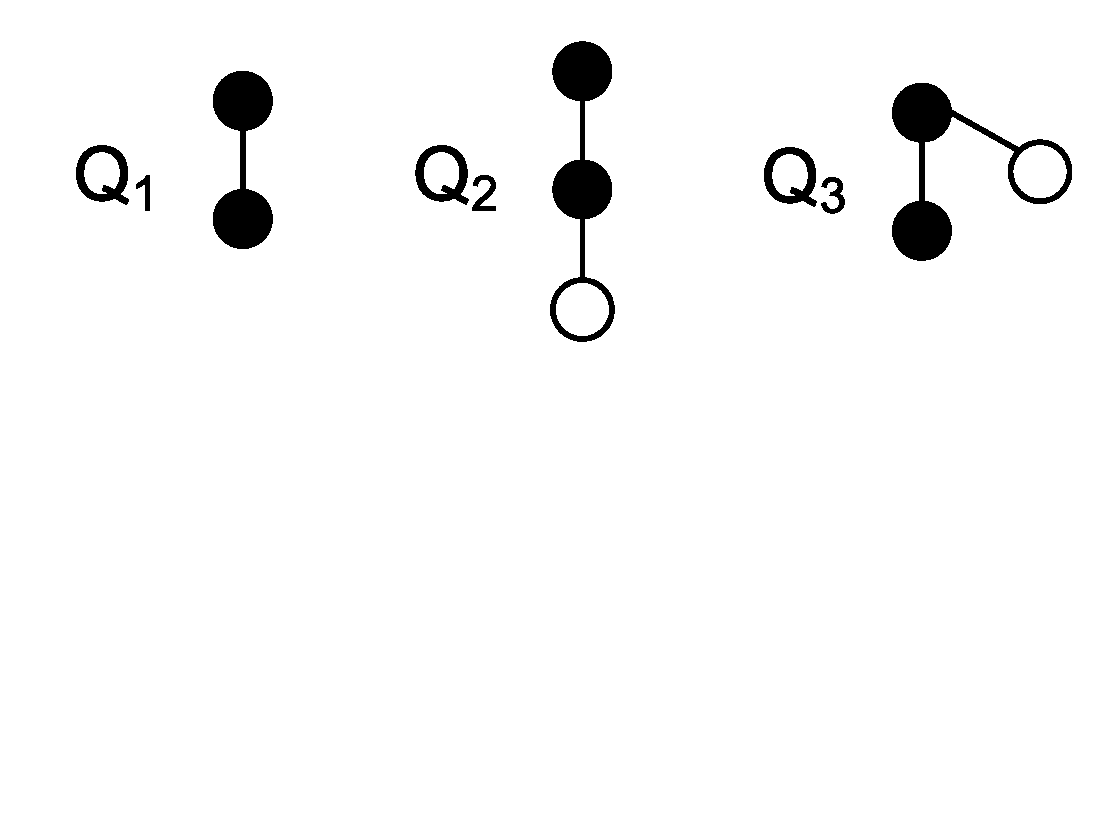
\includegraphics[scale=0.32]{images/ceasing_condition}
	\vspace{-2mm}
	\caption{\scriptsize For 3 subgraphs $Q_1,Q_2,Q_3$, with $\sigma(Q_1)=5$, $\sigma(Q_2)=2$, $\sigma(Q_3)=3$. The current {\sf Top-$k$} set is $\{4,5,6\}$, the input parameters are $k=3$, {\sf Min-sup}$=3$}.
	\label{fig:ceasing_condition}
	\vspace{-6mm}
\end{figure}
\begin{exple}
	In Figure \ref{fig:ceasing_condition}, the minimum element in {\sf Top-$k$} set is $4$, $Q_1$ is the only leaf node at the beginning, i.e. $Leaf(T)=\{Q_1\}$ and $\sigma(Q_1)>4$ so that $Q_1$ can be extended to $Q_2,Q_3$. After extension, $Q_1\notin Leaf(T)$ and $Leaf(T)=\{Q_2,Q_3\}$. $Q_2<$ {\sf Min-sup}, and $Q_3=$ {\sf Min-sup} but $Q_3<4$, and there are already $3$ elements in {\sf Top-$k$} set, i.e. $|Top\_k|=3$. Thus, all the correlation of $Q_2,Q_3$ would not satisfies the condition we want and we cease the search.
\end{exple}



\section{Replica-based Graph Instance Storage}
\label{subsec:replica-storage}

\subsection{Replica Graph Data Structure}
\label{subsubsec:replica-ds}
Considering the large amount of overlaps of the instances in dense graph, we use a novel structure to store a subgraph pattern, which not only get rid of the expensive cost of tackling dense graph, but also be the robust foundation of carrying out an efficient correlation calculation based on instance grouping.
\par Our search tree storage unit is extremely direct and naive. Instead of considering the instances of a pattern, we just create a reproduce of the occurrences of the vertices and the edges of the pattern, called {\bf replica}. We record all the vertex identifications and the edge connections in the replica, we do not record the edge labels.
\begin{figure}[h!]
	\vspace{-2mm}
	\centering
	\subfigure[{\scriptsize Subgraph Pattern $Q$}] {
		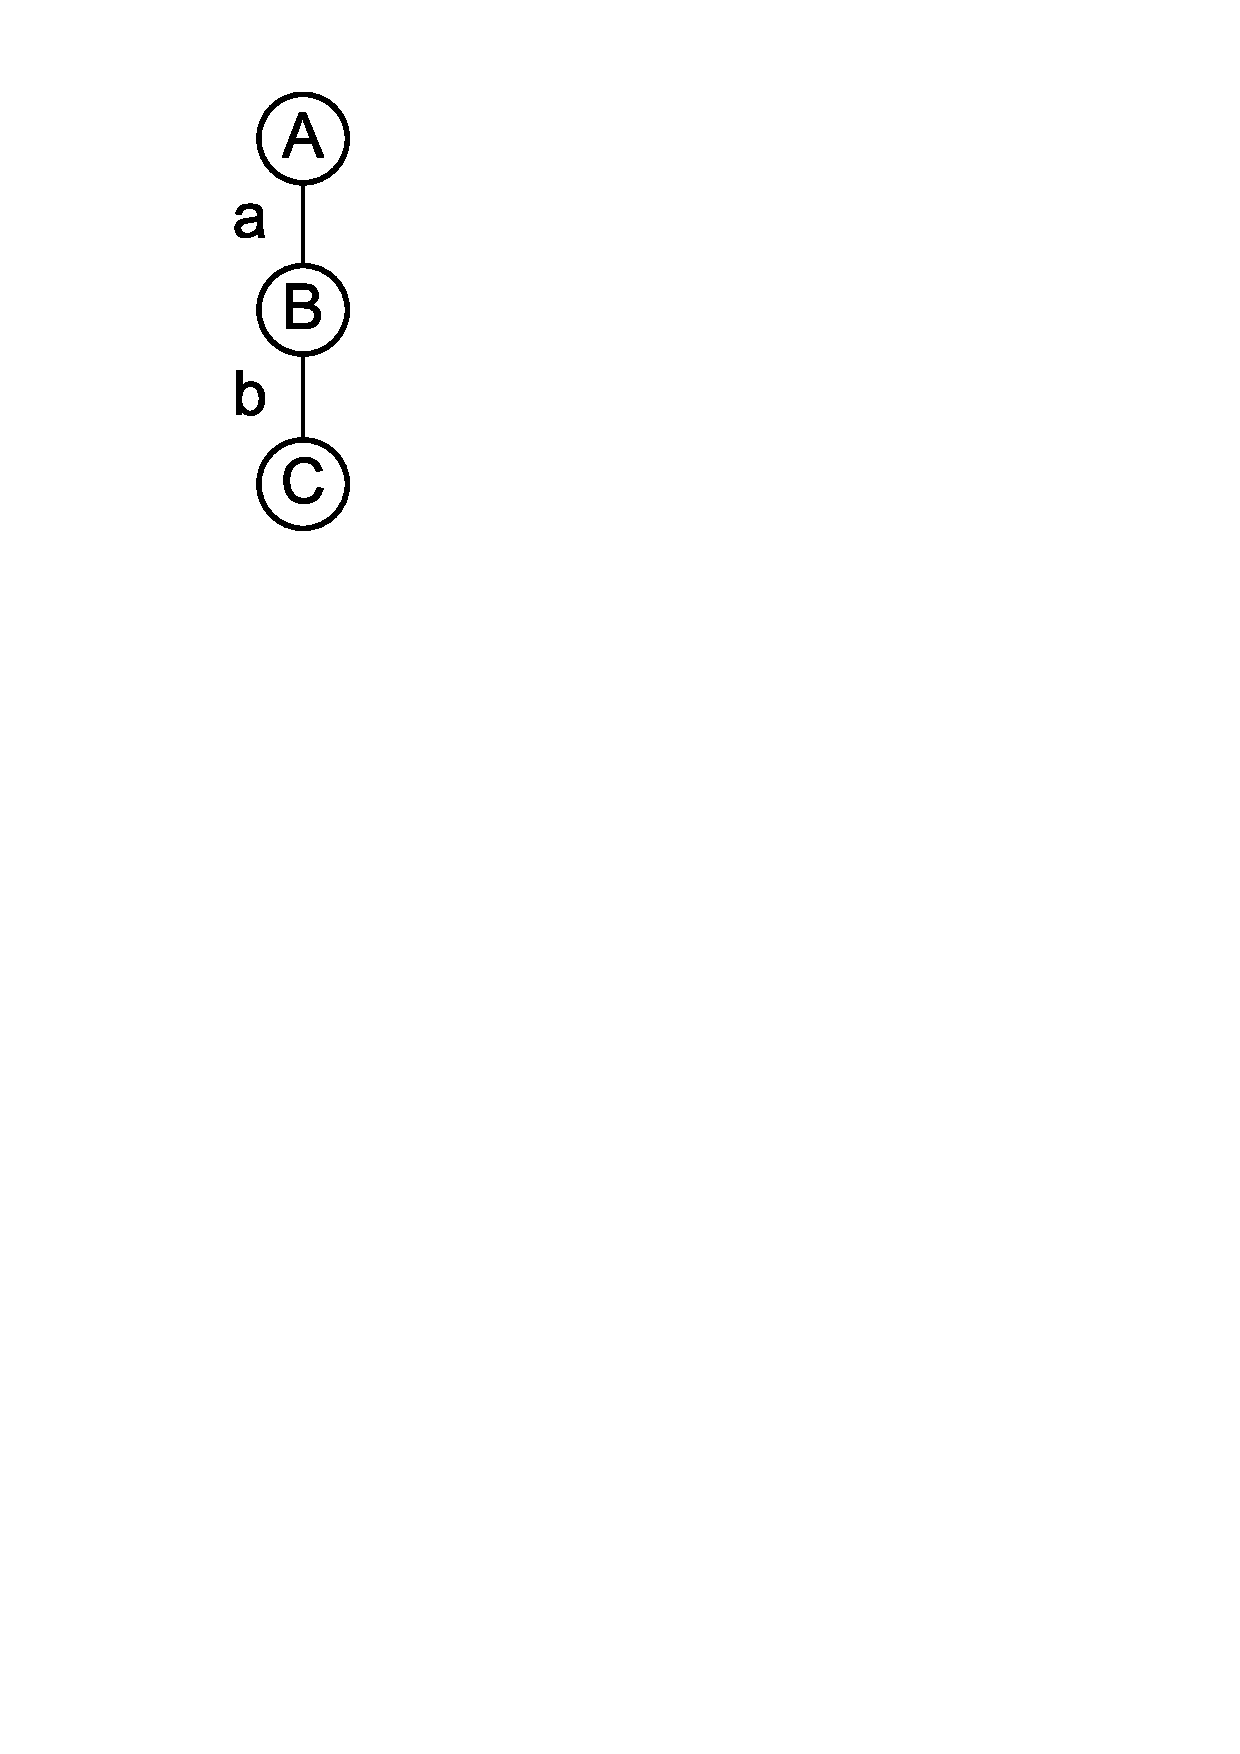
\includegraphics[scale=0.33]{images/replica1}
		\label{fig:replica1}
	}
	\subfigure[{\scriptsize Occurrence of $Q$}]  {
		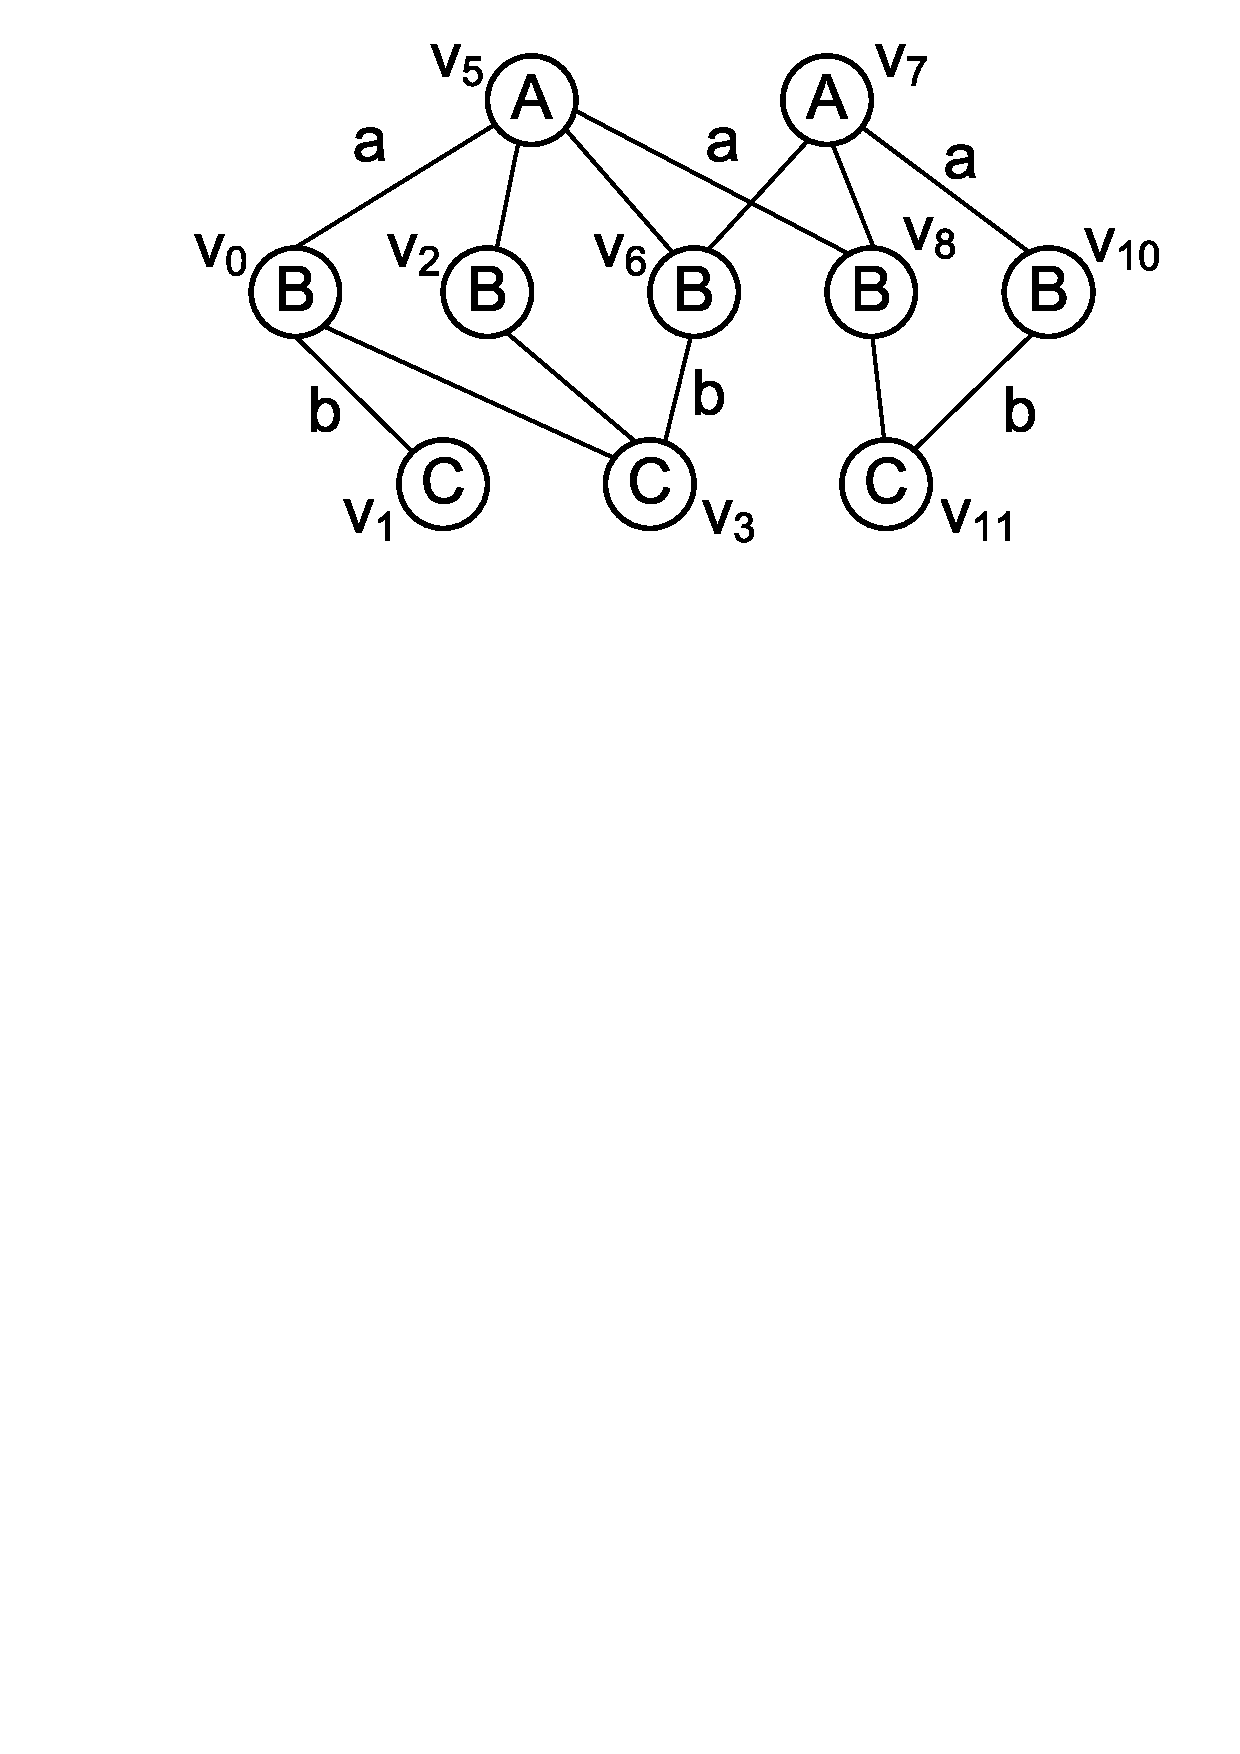
\includegraphics[scale=0.30]{images/replica2}
		\label{fig:replica2}
	}
	\subfigure[{\scriptsize Replica of $Q$}]  {
		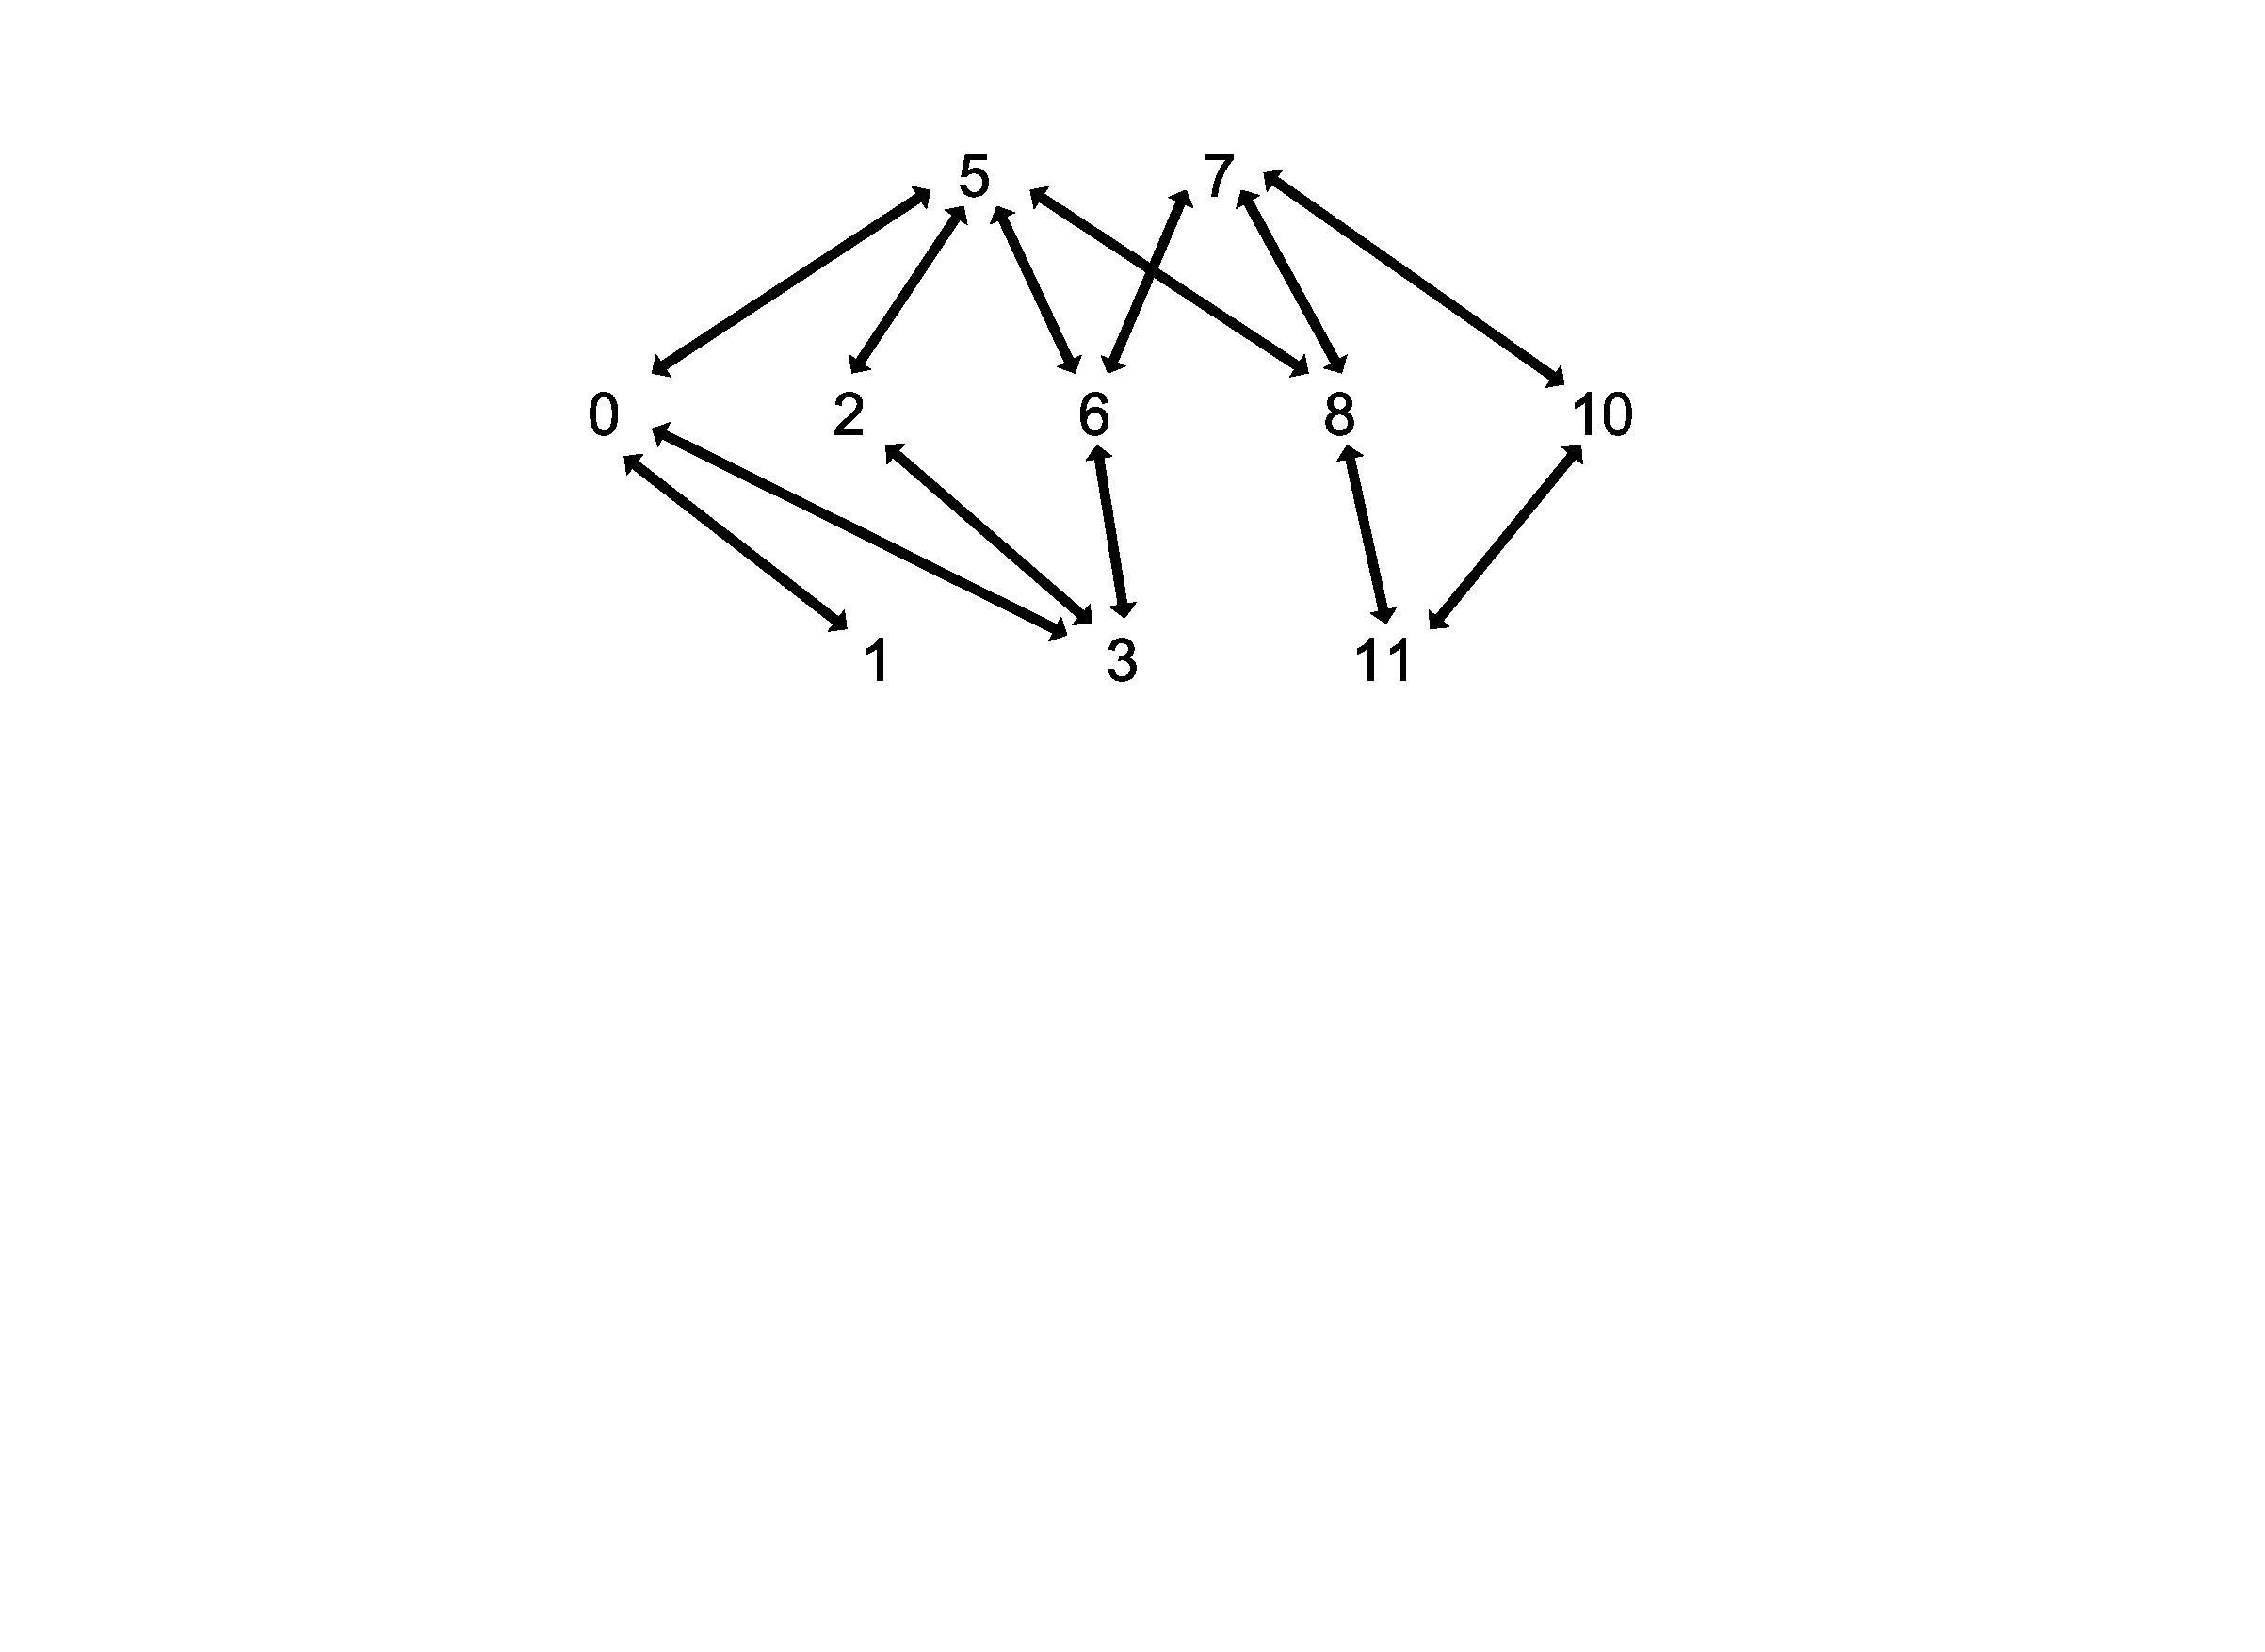
\includegraphics[scale=0.25]{images/replica3}
		\label{fig:replica3}
	}
	\vspace{-2mm}
	\caption{\scriptsize All the edge in Figure \ref{fig:replica2} from $A$ to $B$, $B$ to $C$ has the edge label $a,b$ respectively. Figure \ref{fig:replica3} is replicated from Figure \ref{fig:replica2} without edge labels.}
	\label{fig:replica}
	\vspace{-6mm}
\end{figure}
% \newline
\newline
% As {\sf Found($Q$)} occurs, we store the replica of $Q$ as a unit of the search tree. 
After $Q$ has been $operated$, we remove $replica(Q)$ from memory.

\spara{$\bullet$ Replica Unit.} The illustration of replica is as Figure \ref{fig:replica}. The details of replica is as follows.\\1) For each $Q\in T$, there is a corresponding replica $R(Q)$.\\2) For each $u_i\in Q$, there is a hash-map, $R_i(Q)$, recording the vertex identifications, and $R(Q)=(R_1(Q), R_2(Q), ..., R_{|V_Q|}(Q))$.\\3) For each element $v\in R_i(Q)$, there is a record of all the other vertices which $v$ is connected to in the occurrences of $Q$.

\subsection{Generation of a Replica Graph}
\label{subsubsec:replica-gen}
Algorithms 1 and 2 together describe the complete procedure to construct the replica graph for a subgraph pattern. Replica construction for any pattern $R$ requires knowledge of the replica graph of the pattern $Q$ that is extended to generate it. Henceforth, we refer to such a pattern $R$ as a $child\ pattern$ of $Q$ and $Q$ as the $parent\ pattern$ of $R$. Since the search procedure processes a pattern only after its parent, the replica graph of the $parent\ pattern$ can be used for constructing the replica graph of the $child\ pattern$.
% \begin{algorithm}
% 	\DontPrintSemicolon
% 	\dontprintsemicolon
% 	\KwIn{Training sentences $S_{i}$}
% 	\KwOut{Sentence instances with cost-vectors for training $S_{i,c_i}$}
% 	\SetKwBlock{Begin}{function}{end function}
% 	\Begin($\text{generateCosts} {(} EV_{i,v,r} {)}$)
% 		{
% 	$S_{i,c_{i}} = \left[ \right]$\;
% 		\ForAll{$s \in S, v \in EV $}
% 		{
% 			$c_{i} = \left\lbrace \right\rbrace$\;
% 			set $region \; r = EV_{i,r}$\;
% 			\For{$p \leftarrow 1, properties$}
% 			{
% 				$c_{i,p} \coloneqq cost \left( kb_{r,p},v_{i,r} \right)$\;
% 				\uIf{$c_{p} > Cost_t$}
% 				{
% 					$c_{p} \coloneqq \infty$
% 				}
% 				\Else
% 				{
% 					continue
% 				}
% 			}
% 			\uIf{$\min \left( c \right)  > APE_t$}
% 			{
% 				$c_{i,no\_property} \coloneqq 0$
% 			}
% 			\Else
% 			{
% 				$c_{i,no\_property} \coloneqq \infty$
% 			}
% 			$\text{push} \left( S_{i,c_{i}}, \left( s,c_{i} \right) \right)$
% 		}\label{endfor}
% 		\Return{$S_{i,c_{i}}$}
% 	}
% 	\caption{Cost-Vector Algorithm}\label{costalgorithm}
% \end{algorithm}

\begin{algorithm}
	% \begin{algorithmic}[1] 
	% \REQUIRE input graph: $G$, parent pattern: $Q$, replica of $Q$: $replica(Q)$, extending index: $u$, tuple of extension vertex label and extension edge label: $candidate\ edge$, child pattern: $R$
	% \ENSURE all mappings of child pattern $R$ in $G$ (that is, the replica of $R$: $replica(R)$ in $G$)
	\dontprintsemicolon
	% \KwIn{Graph $G$, parent: $Q$, $replica(Q)$, extending index: $u\in V(Q)$, extension: $candidate\ edge$, child: $R$}
	\nonl \textbf{Input:} Graph $G$, parent $Q$, $replica(Q)$, child $R$, extending index: $u\in V(Q)$, extension: $candidate\ edge (u,v) \in E(R)$\;
	% \KwOut{$replica(R)$}
	\nonl \textbf{Output:} $replica(R)$ \;
	% \SetKwBlock{Begin}{function}{end function}
	% \Begin($\text{generateCosts} {(} EV_{i,v,r} {)}$)
	% {		
	$DFS\ List\leftarrow$ get rooted \textsc{DFS} of $Q$ with $u$ as $root$ \;
	$instance \coloneq \emptyset$\;
	\ForEach{ $u' \in Mappings(u,\ replica(Q))$}
	{
		$instance\leftarrow \{(u,u')\}$ \;
		\ForEach{\textup{edge} $e(u',v')\in E(G)$ \textup{that maps to} $candidate\ edge (u,v)$}
		{
			$instance\leftarrow instance \cup \{(v,v')\}$\;
			$\mathbb{I}\leftarrow$ \textsc{FindAllInstances($R$, $instance$, $\mathbb{I}$, $DFS\ List$, ...)}\;
			\textsc{UpdateReplica($replica(R)$, $\mathbb{I}$, ...)}\;
			$instance\leftarrow instance \setminus \{(v,v')\}$\;
			% Append all edges in $\mathbb{I}$ to $replica(R)$ and update the mappings list for every vertex\;
		}
		$instance\leftarrow instance \setminus \{(u,u')\}$\;
	}
	\Return{$replica(R)$}
	% }
	\caption{\textsc{GetReplica}}\label{algo:search}
	% \end{algorithmic}
\end{algorithm}

Algorithm 1 essentially describes a procedure to find every mapping (also referred to as $instance$) of the $child\ pattern$ in the input graph using the mappings of the $parent\ pattern$ and thus obtain its $replica$ graph. The algorithm begins with a depth-first search ({\sf DFS}) procedure (line 1) executed on the $parent\ pattern\ Q$, selecting the vertex from which the $candidate\ edge$ is extended as the $root$. We call this vertex the $extending\ vertex$ in $Q$. The edges encountered in the depth-first traversal are recorded in an ordered list called the $DFS\ List$, which helps guide the instance enumeration procedure performed subsequently. The algorithm iterates over all mappings of the $extending\ index$ in the $replica$ of the $parent\ pattern$ (line 2) and attempts to enumerate all (if any) instances of the $child\ pattern$ in the data graph one-by-one. More specifically, for every vertex $m$ of $replica(Q)$ that maps to the $extending\ vertex\ u$, the algorithm iterates over its adjacent edges in the input graph that map to the $candidate\ edge$ (line 3) and invokes the {\sf find\ all\ instances} method (Algorithm 2) to enumerate every $instance$ of $child\ pattern\ R$ from $replica(Q)$ that contains this adjacent edge. Algorithm 2, thus invoked, recursively enumerates all instances of $R$ in a depth-first manner following the $DFS\ List$ of $Q$ (computed earlier). In the general case (lines 4-10), the algorithm selects an appropriate graph edge as the mapping of an edge in the $child\ pattern\ R$ (line 5) and recursively invokes the method to find a mapping of the next edge in the $DFS\ List$ that is consistent with the edge mappings selected so far (line 7). Once all edges in the $DFS\ List$ have been mapped to graph edges, the base case (lines 1-3) gets executed where the instance of $R$ thus enumerated is simply returned. Thus, the set of all instances found is returned at the end of Algorithm 2 (line 10) and recorded by Algorithm 1 to update the $replica$ graph (line 6, Algorithm 1). In the update step, the algorithm simply appends all edges of every instance in $\mathbb{I}$ to the existing set of edges of $replica(R)$, and also updates the $mappings\ set$ for every vertex of pattern $R$ to include the vertices of the newly-discovered instances in $\mathbb{I}$.
% The {\sf find all instances()} function used in Algorithm ? is defined below. It enumerates all instances in a depth-first manner starting from the $extending\ index$ as the $root$ by following the {\sf DFS} edge-ordering stored in $DFS\ List$.
\begin{algorithm}
	\dontprintsemicolon
	\caption{\textsc{FindAllInstances} \textsc{(Exact)}}\label{algo:complete-instances}
	\nonl \textbf{Input:} Graph $G$, parent $Q$, $replica(Q)$, child $R$, $DFS$ $List$, partial isomorphism of $R$: $instance$, $\mathbb{I}$\;
	% parent edge: $(u, v)\in E(G)$ mapped to $(u',v')\in E(R)$,
	% \KwOut{$replica(R)$}
	\nonl \textbf{Output:} $\mathbb{I}: $ set of all instances of $R$ in $G$ consistent with input partial isomorphism $instance$\;
	%such that $\forall I \in \mathbb{I} $  $ (u',u),(v',v) \in I$)\;
	% \REQUIRE input graph: $G$, parent pattern: $Q$, replica of $Q$: $replica(Q)$, parent edge: $(u, v)$, $DFS\ List$ of $Q$ rooted at $extending\ index$, child pattern: $R$
	% \ENSURE all mappings of pattern $R$ in $G$ that include $(u, v)$
	\uIf{$|instance|=|V(R)|$}
	{
		\Return{$instance$}
	}
	\Else
	{
		$e(p,c) \coloneq$ \textsc{NextQueryEdge($DFS\ List, ...$)}\;
		$P_{c} \coloneq$ \textsc{FilterCandidates($instance, c, ...$)}\;
		\ForEach{$w \in P_{c}$ \textup{such that w is not yet matched}}
		{
			$instance \leftarrow instance \cup \{(c,w)\}$\;
			$\mathbb{I} \leftarrow \mathbb{I}\ \cup$ \textsc{FindAllInstances($R,instance,$ ...)}\;
			$instance \leftarrow instance \setminus \{(c,w)\}$\;
		}
		\Return{$\mathbb{I}$}\;
	}
	% \IF{all $edges$ in $DFS\ List$ have been mapped}
	% \STATE \textbf{return} $instance$ set
	% \ENDIF
	% \FORALL{adjacent edges $e$ of $v$ in $replica(Q)$}
	% \IF{$e$ maps to the corresponding $child\ edge$ in $DFS\ List$ \textbf{and} \textbf{not} already in $instance$}
	% \STATE $instance\leftarrow instance\cup e$
	% \STATE $\mathbb{I}\leftarrow \mathbb{I}\ \cup\ ${\sf find\ all\ instances($R$, $e$, $instance$, $DFS\ List$)}
	% \STATE $instance\leftarrow instance \setminus e$
	% \ENDIF
	% \ENDFOR
	% \STATE \textbf{return} $\mathbb{I}$
\end{algorithm}

This replica storage strategy not only builds a foundation for the sequential efficient correlation calculation, but also benefits the MNI support counting in the single large graph since we can directly get $\sigma(R)$ when we record the replica of $R$ just by counting all the sizes of the images $M(v)$, where $v\in R$.


\subsection{Indexing to Facilitate Replica Deletion}
\label{subsubsec:replica-indexing}

\section{Subgraph Extension}
\label{subsec:subgraph-ext}
\subsection{Extension Rule}
We subscript the node patterns in a subgraph patterns to identify their order of discovery.
\begin{defn}[Vertices Subscripting]
	Let $Q$ be a frequent subgraph in $T$, apart from vertex identification $v_i$, we use another metric to subscript the vertices in $Q$ by the order we discover the pattern $Q$, denoted as $S_Q=(s_0,s_1,...,s_n)$, where $n=|V_Q|$. And for $s_i$ and $s_j$, if $i<j$, then the vertex $v_i$ is discovered earlier than the vertex $v_j$.
\end{defn}
Taking advantage of subscripting, it is easy to get the right-most path of a subgraph. Then, we only grow the new vertices in right-most path. Corresponding to the best-first-search strategy, the node with highest MNI support will be chosen, suppose $Q$. Then, for all the vertices in its right-most path of the replica of $Q$, we try one edge extension from them respectively, see Algorithm \ref{algo:extension}.

\begin{algorithm}
	\dontprintsemicolon
	% \begin{algorithmic}[1]
	\nonl \textbf{Input:} Graph $G$, parent $Q$, $replica(Q)$ \;
	\nonl \textbf{Output:} $Ex(Q)$: set of candidate edge extensions for $Q$\;
	% \REQUIRE data graph $G$, subgraph pattern $Q$, replica of $Q$, {\sf Min-sup}
	% \ENSURE frequent pattern set extended from $Q$, $Ex(Q)$
	$Ex(Q)\coloneq \emptyset$ \;
	$rmpath \leftarrow$ right-most path of $Q$ from $DFS\ Code(Q)$\;
	\ForEach{$v\in rmpath$}
	{
		\ForEach{$v'\in Mappings(v,replica(Q))$}
		{
			$E\leftarrow$ set of all edges $(v',w')\in E(G)$ extending $Q$\;
			$Ex(Q)\leftarrow Ex(Q)\cup E$
		}
	}
	\Return{$Ex(Q)$} 
	% \STATE $Ex(Q)\leftarrow\emptyset$
		% \STATE $Rmpath\leftarrow$ right-most path of $Q$
		% \FORALL{$s$ in $Rmpath$}
		% \STATE $Ex(Q)\leftarrow Ex(Q)\cup$ possible extensions
		% \ENDFOR
		% \FORALL{$ex$ in $Ex(Q)$}
		% \IF{$\sigma(ex)<$ {\sf Min-sup}}
		% \STATE $Ex(Q)\leftarrow Ex(Q)\setminus ex$
		% \ENDIF
		% \ENDFOR
		% \RETURN $Ex(Q)$
	% \end{algorithmic}
	\caption{\textsc{SubgraphEdgeExtensions}}\label{algo:extension}
\end{algorithm}

\subsection{Duplicated Subgraph Prunning}
To avoid the duplicated subgraph judgement, we take the advantage of the DFS code, and the minimum DFS code in gSpan\cite{YH02}, whenever a subgraph is founded, we get its DFS code, denoted as $C(Q)$ and remodel this subgraph by using this code. Then, we build the minimum DFS code of this subgraph $Q$. This minimum DFS code, denoted as $Z(Q)$ is the canonical label of this subgraph in our definition.

\par We use a dictionary $\mathbb{D}$ to store all the minimum DFS code we have discovered so far. When a subgraph $Q$ is discovered and its graph code $C(Q)$ has been transformed to minimum DFS code $Z(Q)$, we search $Z(Q)$ in the dictionary. If $Z(Q)\in \mathbb{D}$, then $Q$ must have been discovered before, so we prune $Q$.


\section{Correlation Computation}
\label{subsec:corrcomp}

\subsection{Global Index}
\label{subsec:global-index}

We use a global index to record all the distance information. Each vertex of the data graph stores two catogories of distance information.

\squishlist
\item{\bf Proximity Vertices.} For each $u\in G$, we store the information of proximity vertices of $u$, denoted as $CorV(u)$, for each vertex $u\in CorV(u)$, there exists $d(u,v)\le h$.
\squishend
\squishlist
\item{\bf Proximity Patterns.} For each $u\in G$, we store the information of proximity patterns of $u$, denoted as $CorP(u)$, for each pattern $Q\in CorP(u)$, suppose the instance-groups of $Q$ is $\mathbb{I'}=\{I'_1,I'_2,\ldots,I'_{\sigma(Q)}\}$, there exists $I'\in \mathbb{I'}$, $\exists v\in I'$, $d(u,v)\le h$.
\squishend
With the global index acquired before the search, there is no need to consider anything about the distance (hop-constraints) in the search steps. The detail of the maintenance of these two indices is specified in Section \ref{subsec:calculating}.

\subsection{Calculating Correlation}\label{subsec:calculating}
\begin{defn}[Positive Instance Group]
	Given two subgraphs $Q_1$ and $Q_2$ in the input graph $G$, their instance-groups
	$\mathbb{I'}=\{I'_1,I'_2,\ldots,I'_{\sigma(Q_1)}\}$ and $\mathbb{J'}=\{J'_1,J'_2,\ldots,J'_{\sigma(Q_2)}\}$,
	respectively, and a user-defined distance-threshold $h$, assume that $\sigma(Q_1) \le \sigma(Q_2)$.
	Then, we say an instance group of $Q_1$, $I'_i\in \mathbb{I'}$ is a {\bf positive instance group} of $Q_2$ if following condition is satisfied.
	%
	\begin{align}
		\exists J' \in \mathbb{J}, \exists u \in I', \exists v \in J', d(u,v)\le h
	\end{align}
	Then, we denote $P(I'_i,Q_2,h)=1$, otherwise $P(I'_i,Q_2,h)=0$.
\end{defn}
\begin{thrm}
	Let $Q_1,Q_2$ be two subgrpah patterns, and an instance group of $Q_1$, $I'$. Then,	if $Q_2\in \cap CorP(v),v\in I'$, $P(I'_i,Q_2,h)=1$.
	otherwise, $P(I'_i,Q_2,h)=0$.
\end{thrm}
The process of correlation calculation could be considered as a {\bf collection}. Suppose we are calculating the correlation of $Q_1$, i.e. $\tau(Q_1,Q_k,h)$, for all $Q_k\in Cor(T)$. Taking advantage of the global index in Section \ref{subsec:global-index}, by traversing all the vertices in a group can we know the correlation $\tau()$ of all the $v$. We collect these sets one-by-one and finally we could know all the correlation of $Q_1$, i.e. $\tau(Q_1,Q_k,h)$, for all $Q_k\in Cor(T)$.

\subsection{Replica Structure Transformation}
It is more convenient to implement an efficient collection in a hierarchical structure, like tree. As a result, to initialize a collection, we first transform the search space of the collection to a particular tree.
\par Prior to the detailed operations, we first define the group center and the collection tree of a pattern.
\begin{defn}[Group Center and Center Subscript]
	Given a subgraph $Q$, and the instance-groups of $Q$, $\mathbb{I'}=\{I'_1,I'_2,\ldots,I'_{\sigma(Q)}\}$, a group center $u$ of $I'_i$ is the vertex having the minimum MNI support among all $v\in I'_i$, denoted as $u=center(I_i)$, a center subscript is the vertex subscript has the MNI support of the images, denoted as $centerSubscript(Q)$. i.e. $centerSubscript(Q)=i$, where $M(s_i)=\sigma(Q)$.
\end{defn}
\begin{defn}[Collection Tree]
	Given a subgraph $Q$, a collection tree of $Q$, $CT(Q)$ is tree transfromed from the tree structure replica, and rooted at $centerSubscript(Q)$.
\end{defn}
% First of all, if a subgraph contains any backward edges, we remove all its backward edges in its replica prior to the calculation. This is because 1) removing backward edges would not affect the result of correlation calculation. 2) removing backward edges could derive a tree structure subgraph, which is more convenient to carry out the collection.
\begin{figure}[t!]
	\vspace{-2mm}
	\centering
	\subfigure[{\scriptsize Subgraph Pattern $Q_1$}] {
		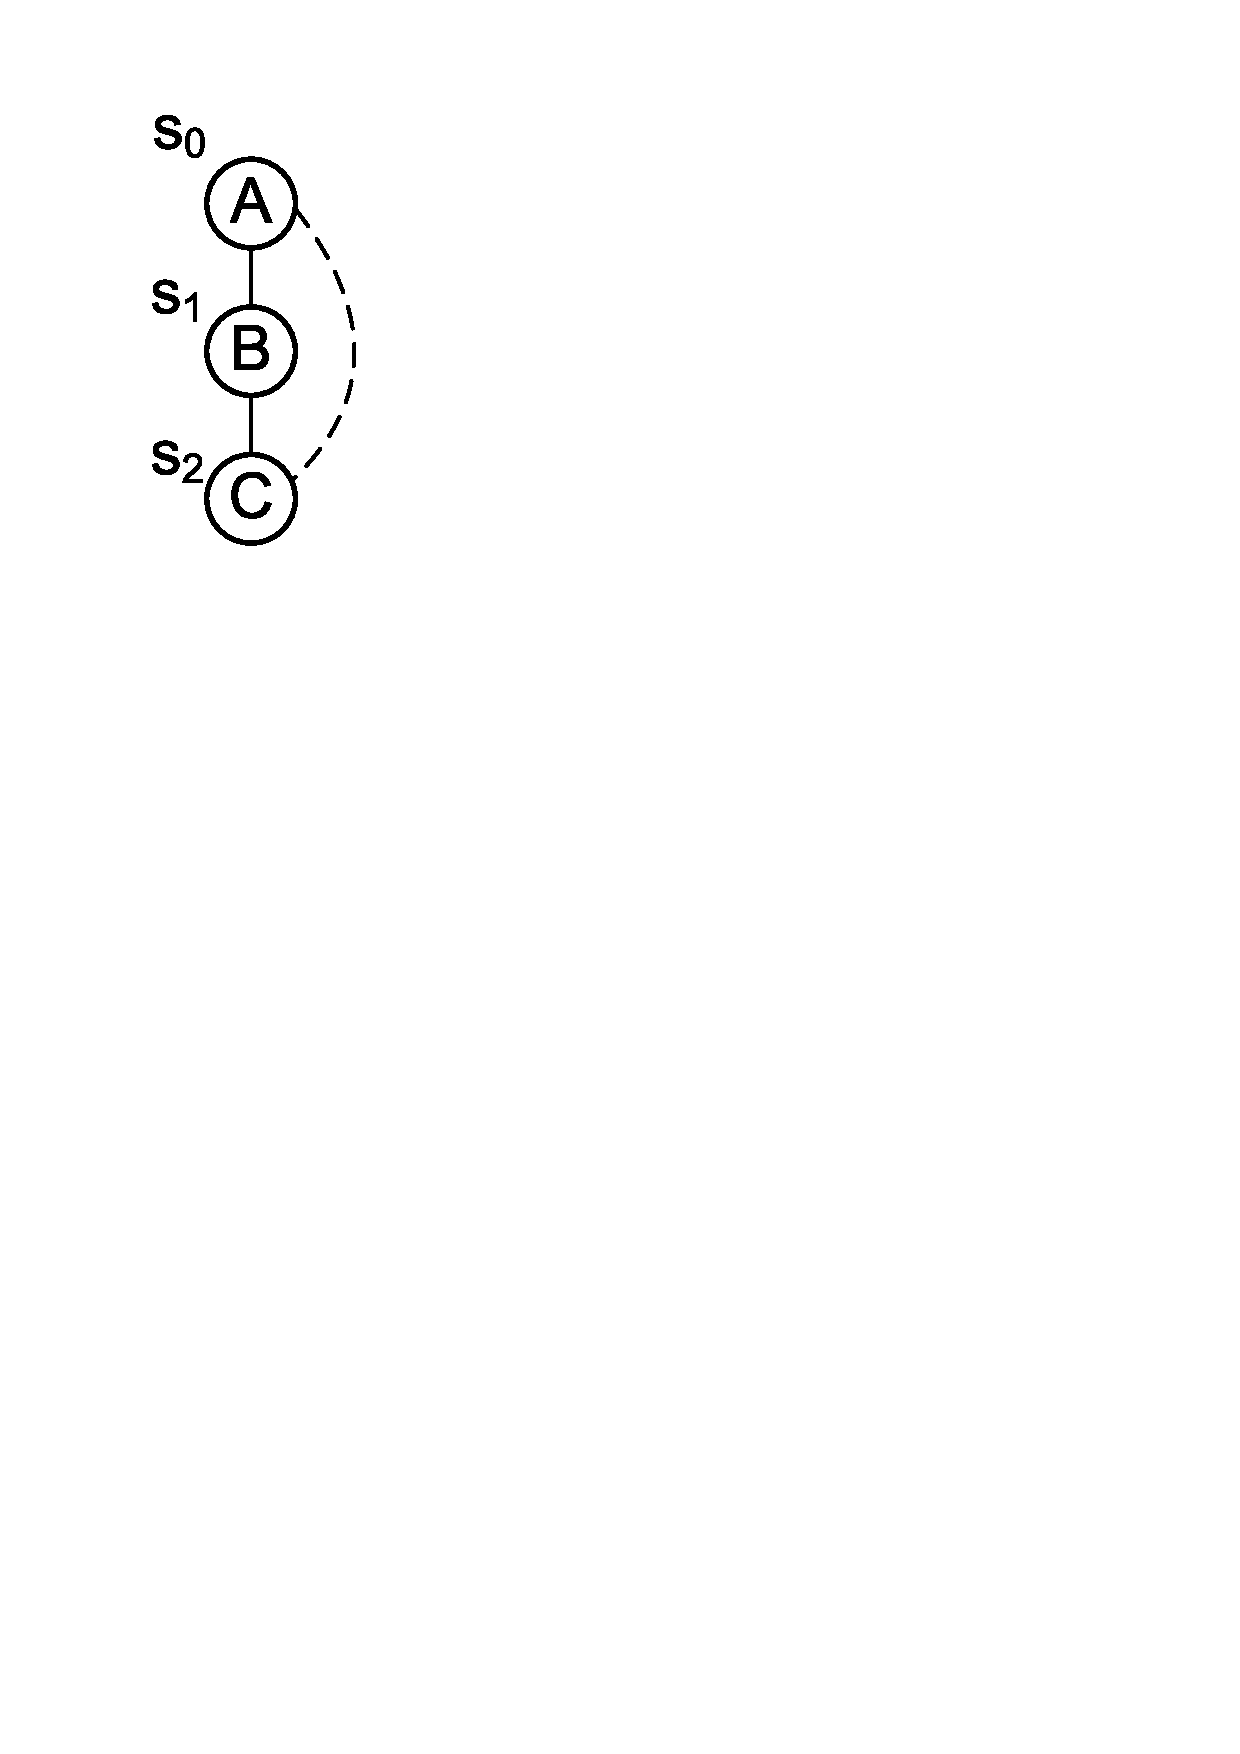
\includegraphics[scale=0.35]{images/tree_structure0}
		\label{fig:tree_structure0}
	}
	\subfigure[{\scriptsize Occurrence of $Q_1$}] {
		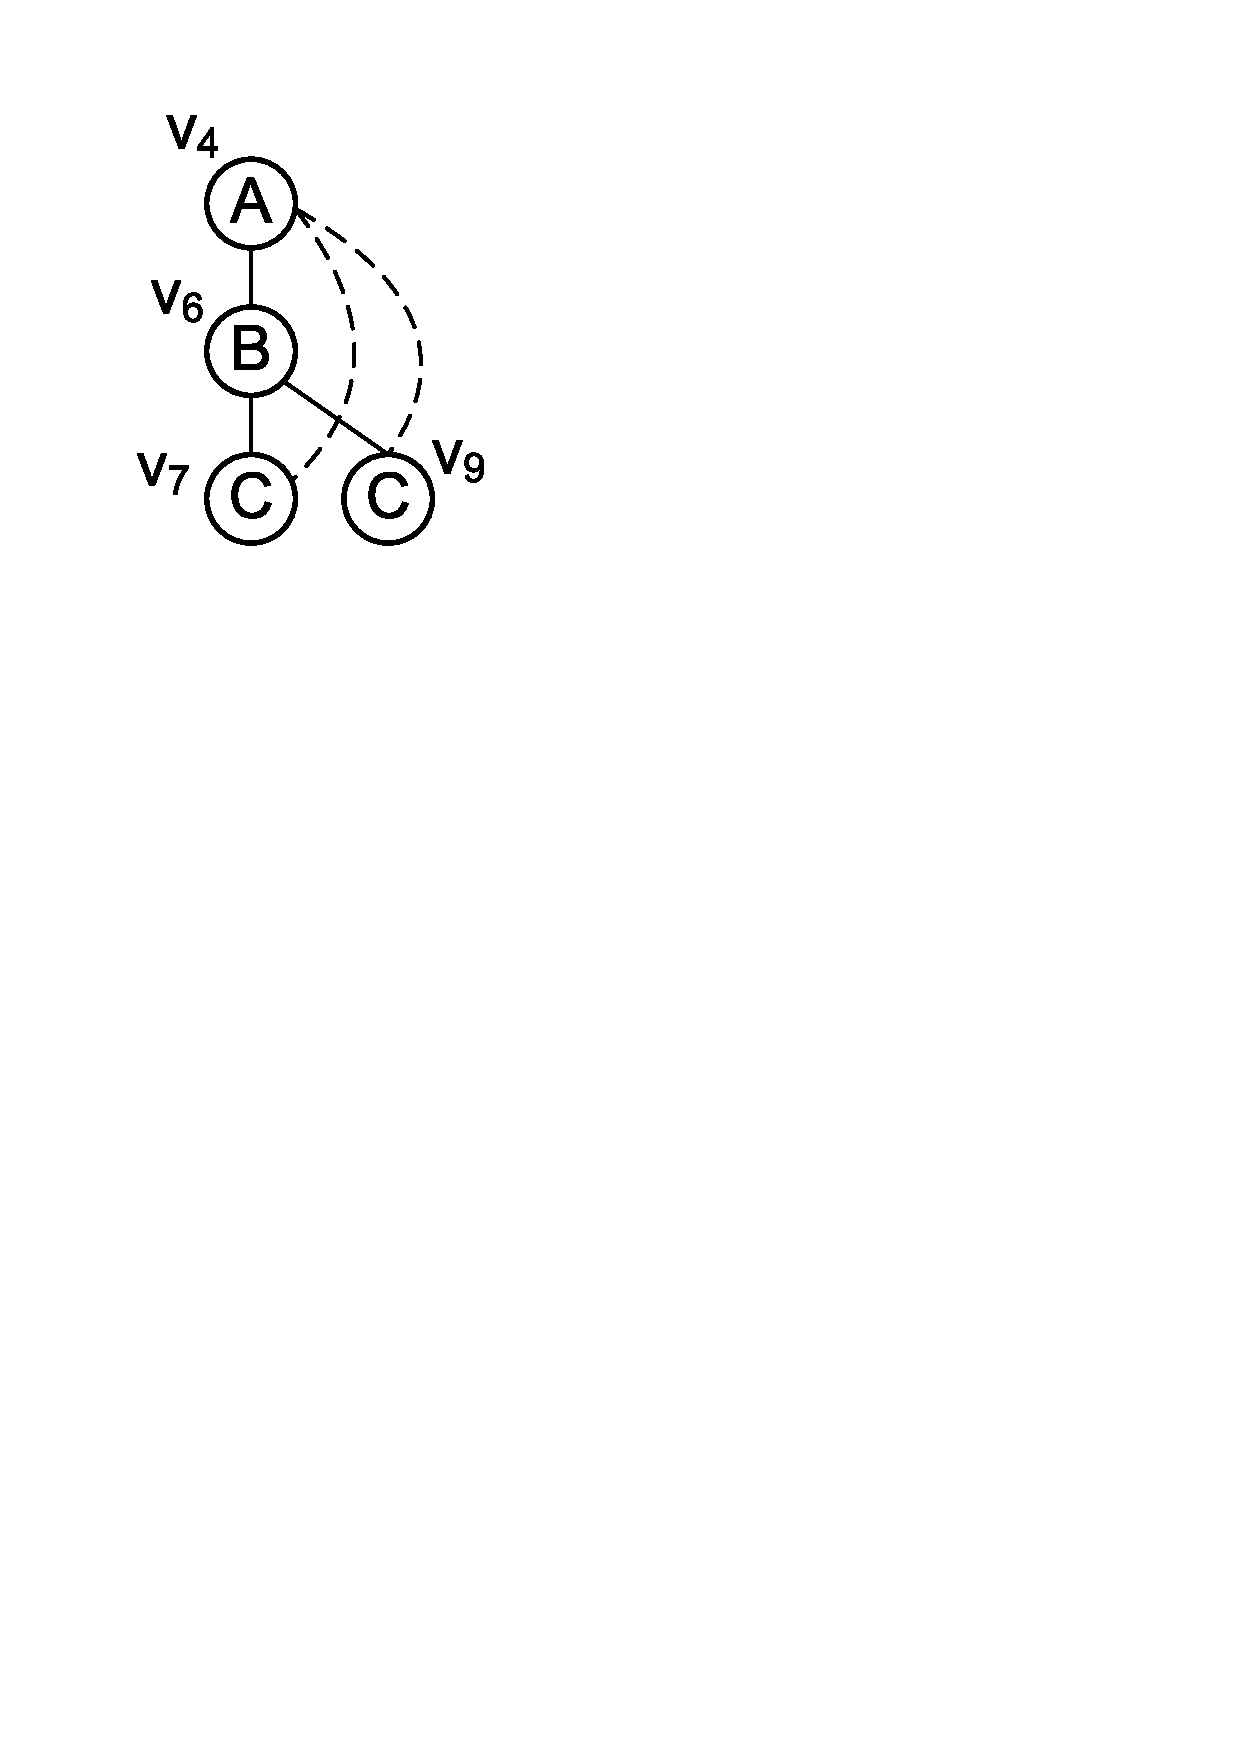
\includegraphics[scale=0.35]{images/tree_structure1}
		\label{fig:tree_structure1}
	}
	\subfigure[{\scriptsize Replica of $Q_1$}]  {
		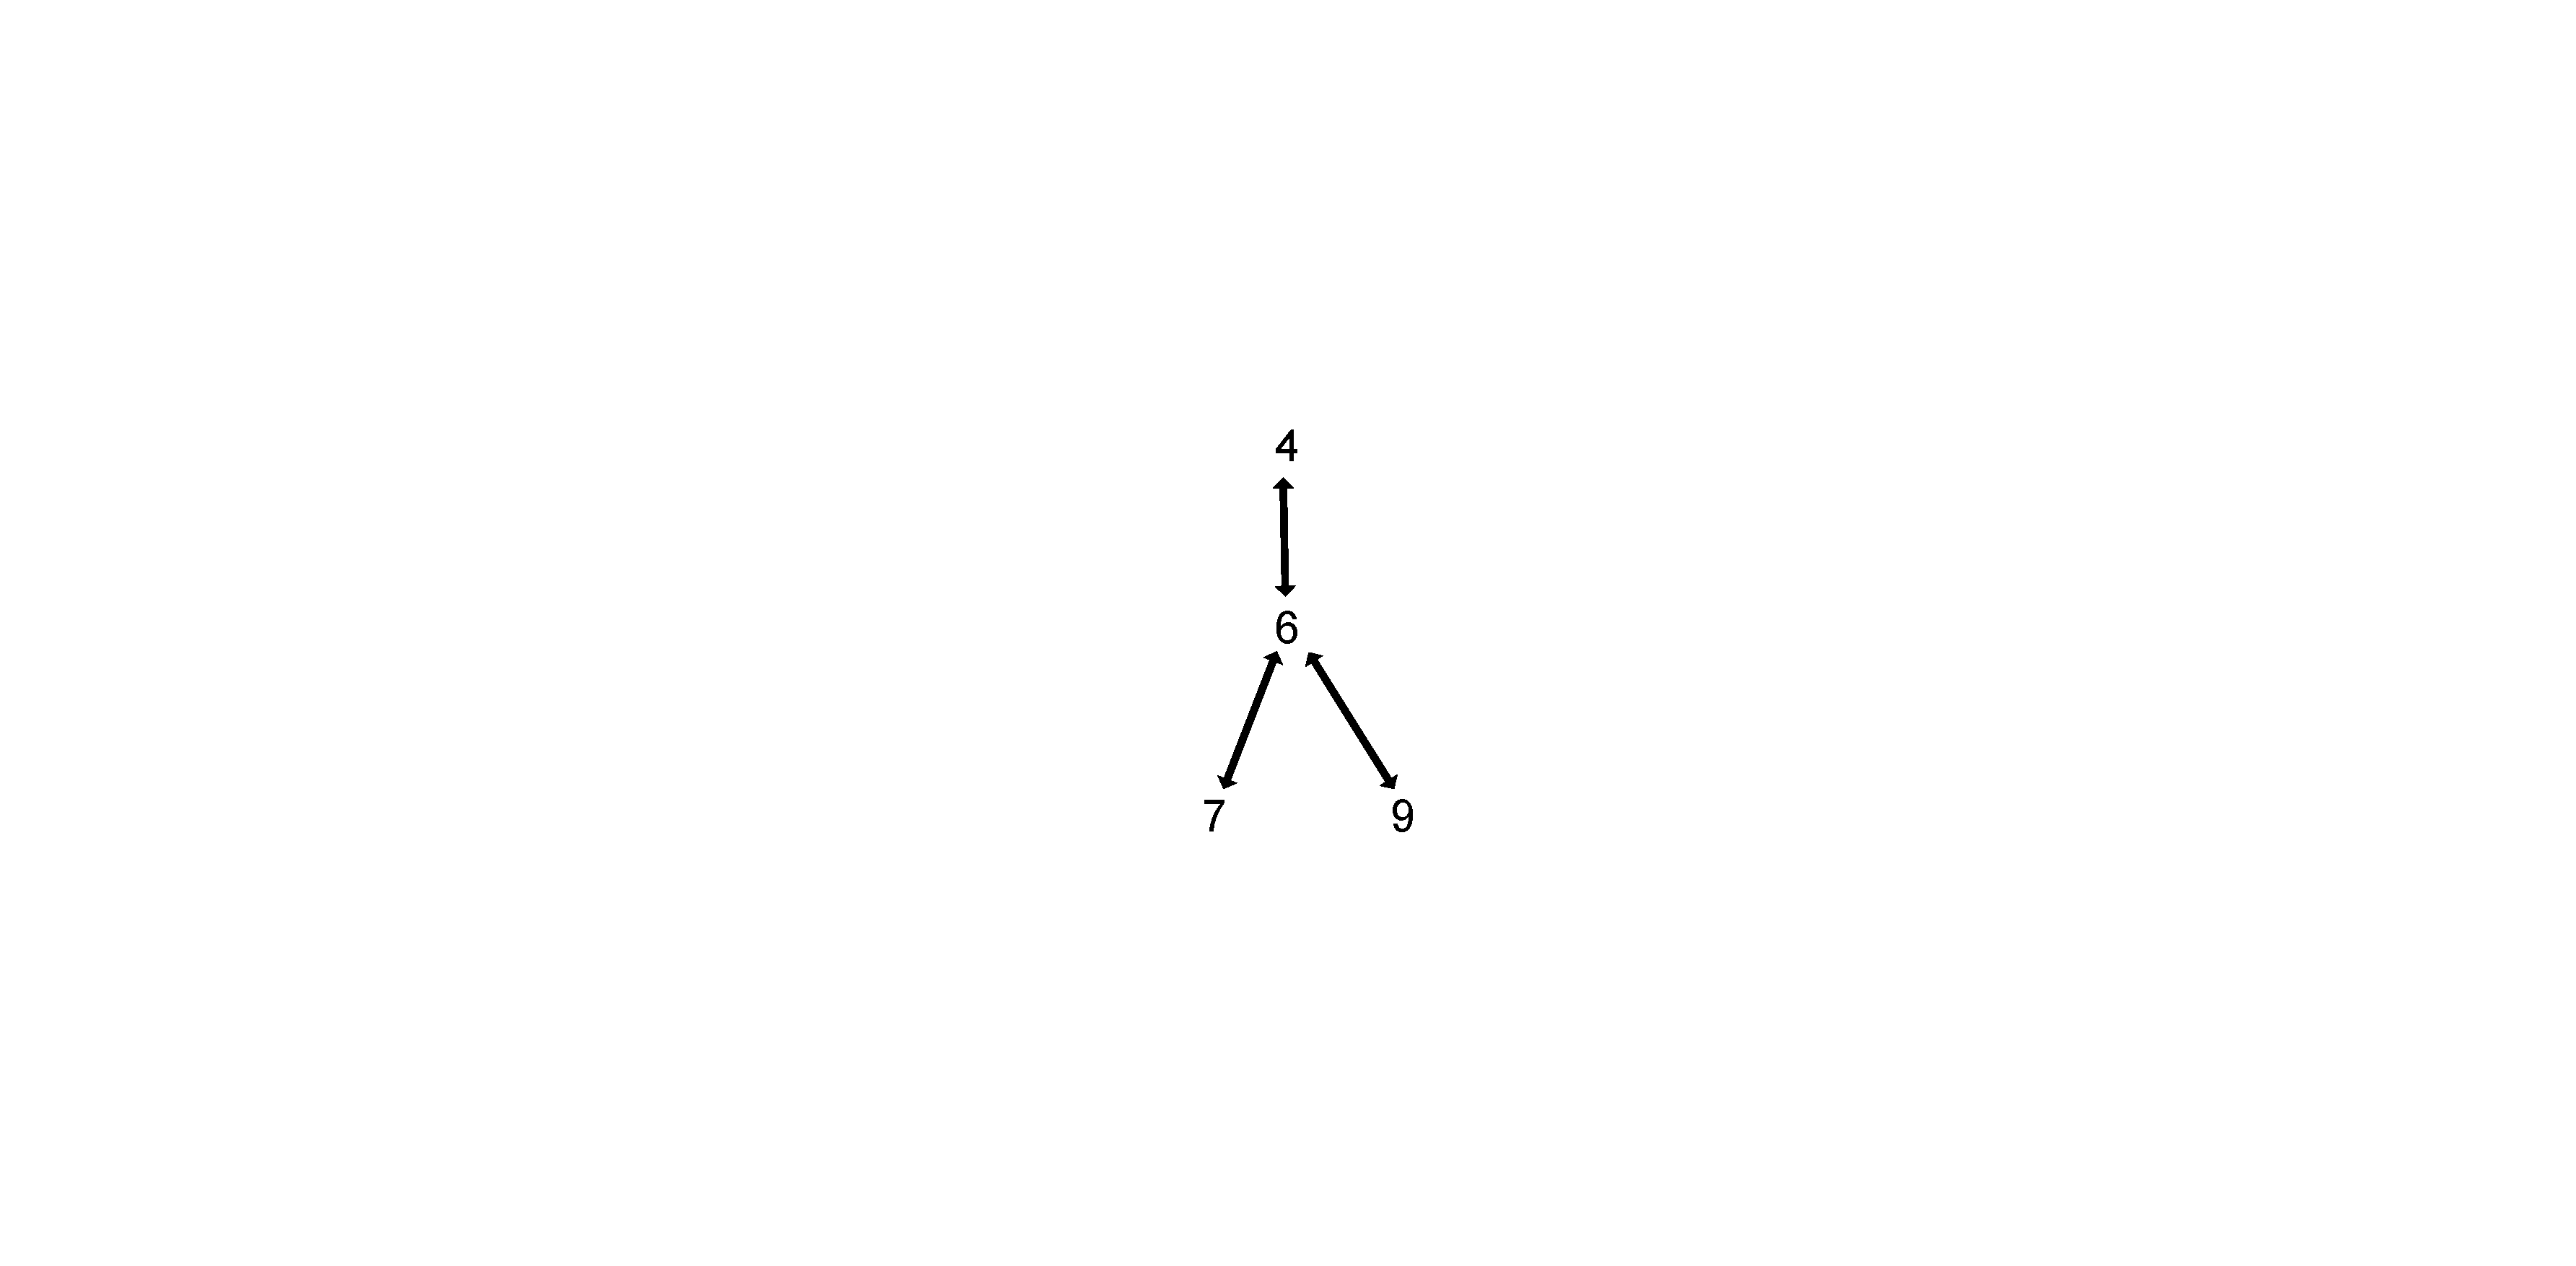
\includegraphics[scale=0.26]{images/tree_structure2}
		\label{fig:tree_structure2}
	}
	\subfigure[{\scriptsize Subgraph Pattern $Q_2$}]  {
		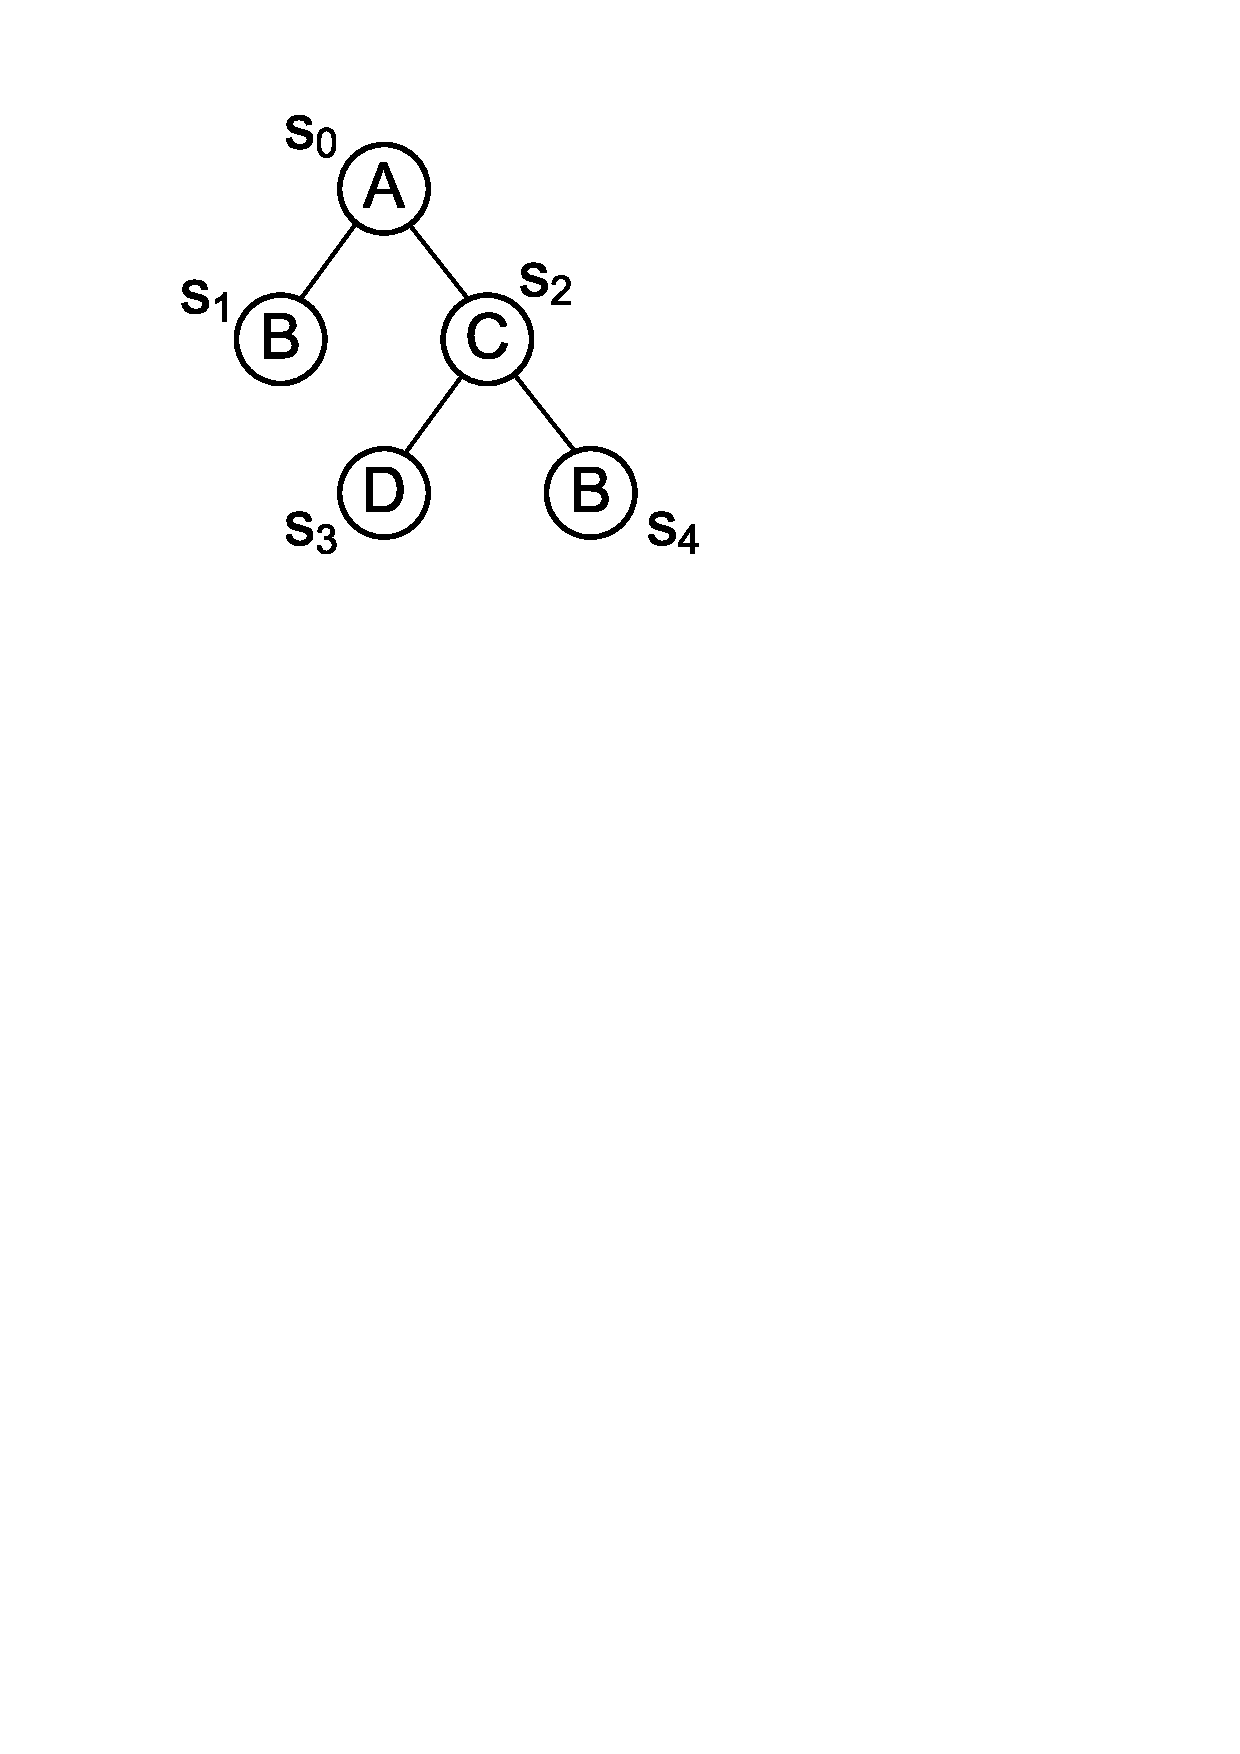
\includegraphics[scale=0.33]{images/tree_structure3}
		\label{fig:tree_structure3}
	}
	\subfigure[{\scriptsize Collection Tree of $Q_2$}] {
		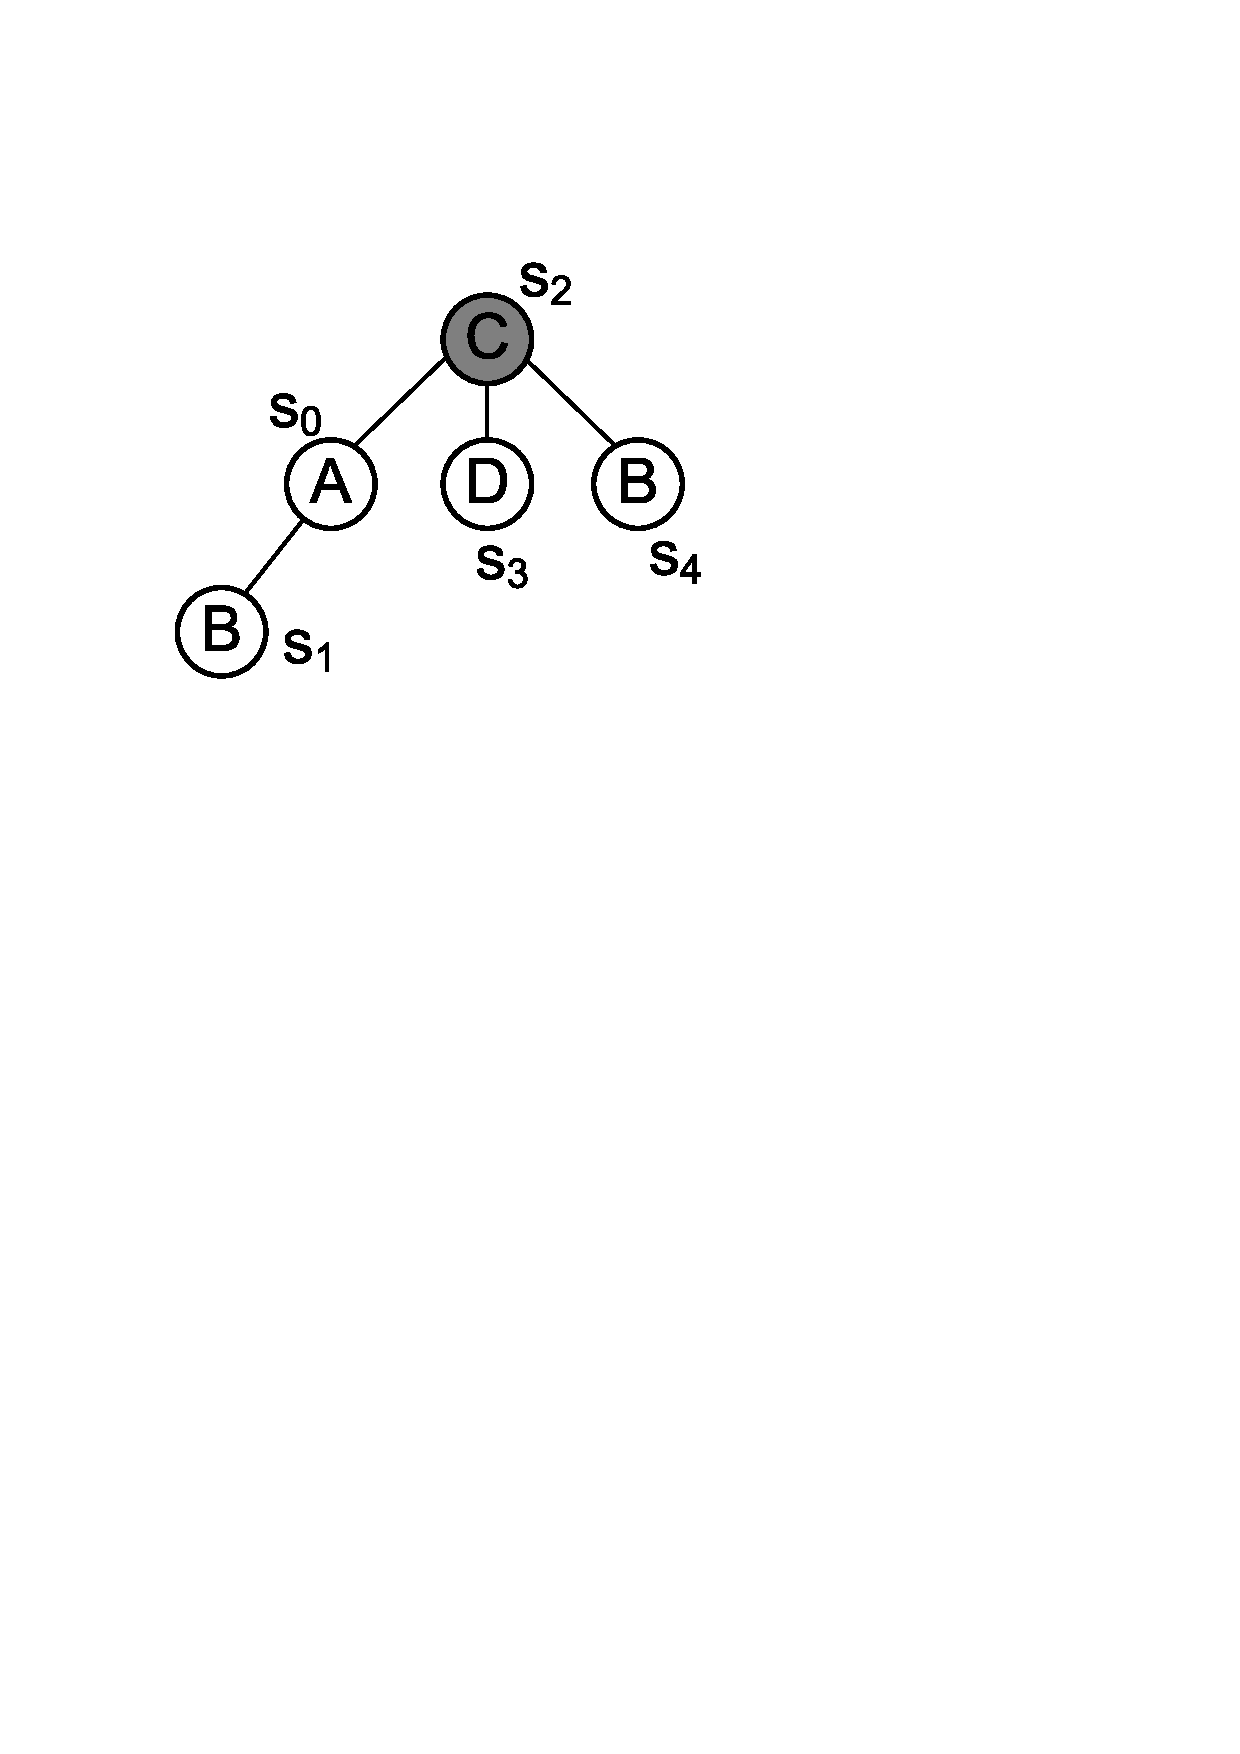
\includegraphics[scale=0.33]{images/tree_structure4}
		\label{fig:tree_structure4}
	}
	\subfigure[{\scriptsize Occurrence of $Q_2$ in $G$}] {
		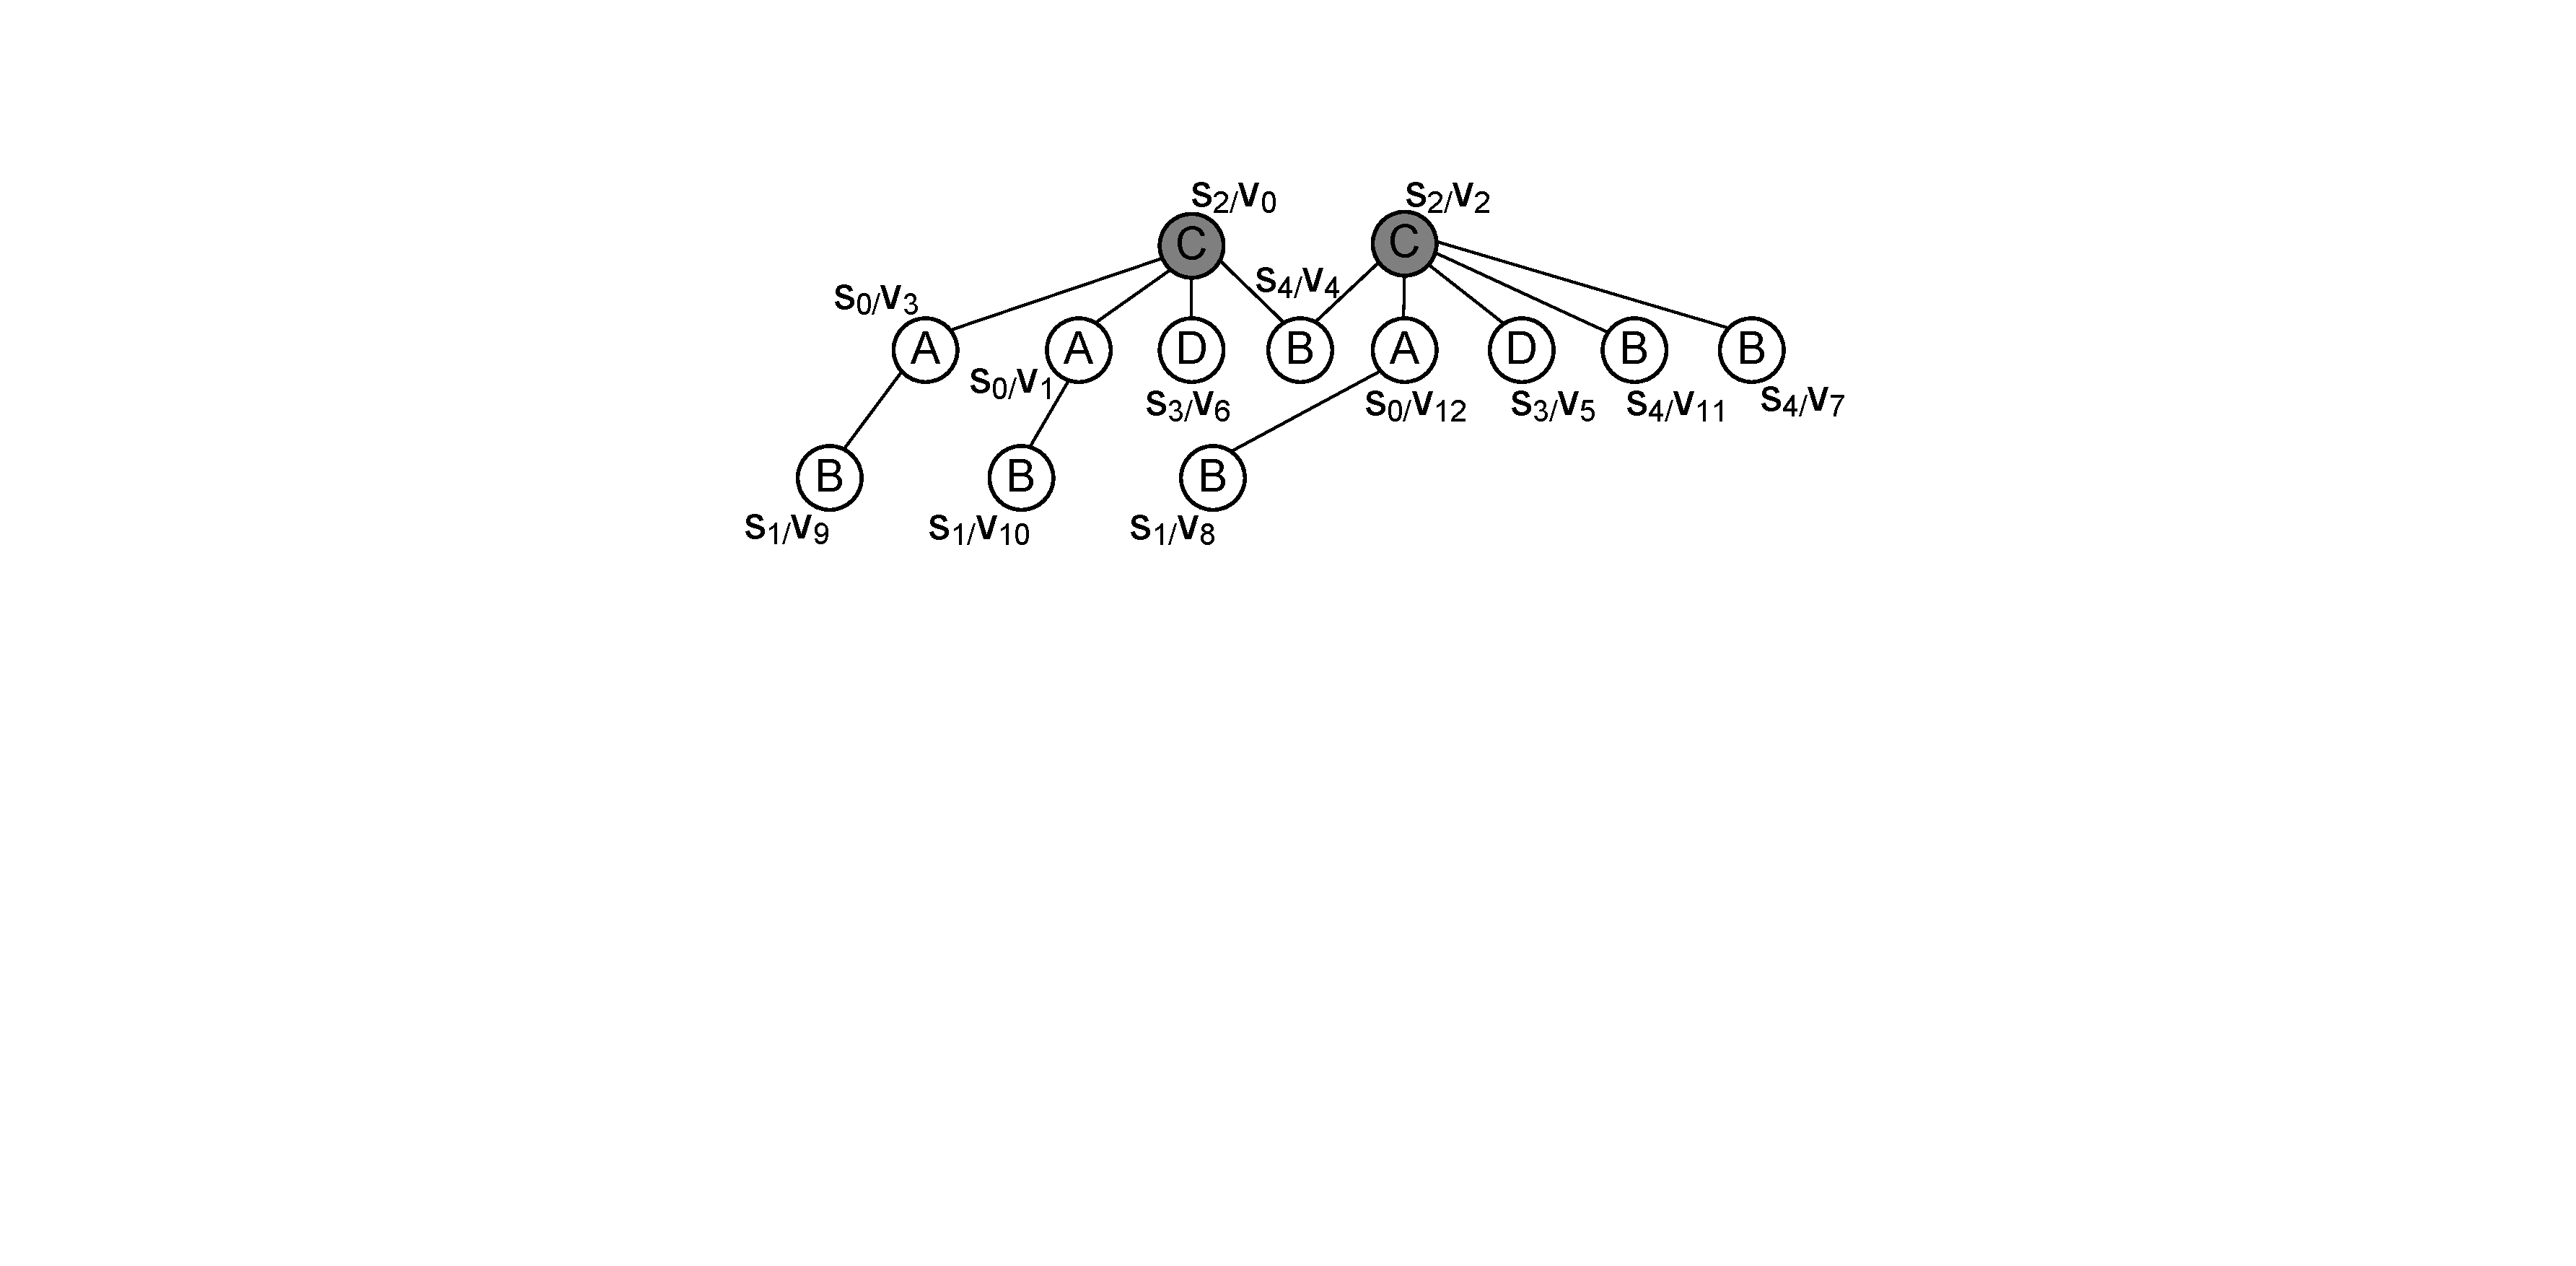
\includegraphics[scale=0.30]{images/tree_structure5}
		\label{fig:tree_structure5}
	}
	\vspace{-2mm}
	\caption{\scriptsize Figure \ref{fig:tree_structure0} is the subgraph pattern of $Q_1$, Figure \ref{fig:tree_structure2} is a replica of the occurrence of $Q_1$ in Figure \ref{fig:tree_structure1} without any backward edges (the dotted lines are the backward edges in $Q_1$). Figure \ref{fig:tree_structure4} is the same subgraph pattern $Q_2$ with Figure \ref{fig:tree_structure3}, with collection tree rooted at the group center $s_2$. Figure \ref{fig:tree_structure5} is the occurrence of $Q_2$ in data graph $G$.}
	\label{fig:replica}
	\vspace{-6mm}
\end{figure}
~\newline
~\newline

%
Then, we consider the group center as the root of the tree. During the collection, the collection is initiated from the root of the tree.

% \subsubsection{Recursive Collection}\label{subsubsec:recursive}
% The collection could be completed by a naive straight forward traversal. However, we traverse by top-bottom manner and collect by bottom-top manner. This manner could help us to reduce duplicated calculation by saving the information of all ones subtrees.

\par Prior to the correlation computations for $Q$, we first update the distance index of proximity patterns using the data of proximity vertices. That is, for all $u\in Q$, for each $v\in Cor(u)$, $CorP(v)=CorP(v)\cup Q$.
\begin{lma}
	\label{lemma:distance bidirection relation between vertices and patterns}
	Let $Q$ be a subgraph, for all $v$ in data graph $G$, if $v\in \cup CorV(u),u\in Q$, then there must exists $Q\in CorP(v)$.
\end{lma}
\par After the update of the distance index, we operate the correlation calculation of subgraph $Q$. This process includes two phases.

\spara{$\bullet$ Collection Phase:} For each group center $c\in Center(Q)$, all instances of $Q$ including $c$ are enumerated in a depth-first manner similar to the recursive instances-enumeration technique of Algorithm 2. A set union of patterns contained in $CorP(u)$ is performed across every vertex $u$ of an instance group. At the same time, every vertex $v$ in the $proximity\ vertices\ map$ of $u$ ($CorV(u)$) records the proximity of pattern $Q$ in its $proximity\ patterns\ map$ ($CorP(v)$).

\begin{align}
	Collect(c,Q)=\cup \{CorP(v)|v\in instance group\}
\end{align}
% Eventually, every group center has all the correlation corresponding to the collection tree.

\spara{$\bullet$ Computation Phase:} The correlation between patterns $Q_1$ and $Q_2$ is easily stated by calculating the count of instance groups of $Q_1$ that are positive instance group of $Q_2$.
\par Clearly, a instance group $I'_i$ of $Q_1$ is a positive instance group $Q_2$, i.e. $P(I'_i,Q_2,h)=1$ if and only if
\begin{align}
	u=groupCenter(I'_i), Q_2\in Collect(u,Q_1)
\end{align}
Then, we sum all the results to get the correlation.
\begin{align}
	\tau(Q_1,Q_2,h)=\sum_i^{\sigma(Q_1)} P(I'_i,Q_2,h)
\end{align}
Algorithm 4 summarises the steps described above.

\begin{algorithm}%[h!]
	\caption{\textsc{Operate}}\label{algo:operate}
	% \begin{algorithmic}[1]
		\dontprintsemicolon
		\nonl \textbf{Input:} Graph $G$, $Q$, $replica(Q)$, hop $h$, $CorV$, $CorP$\;
		\nonl \textbf{Output:} $\tau({Q,Q_{k},h})$, updated {\sf Top\ $k$} order\;
		% $DFS\ List\leftarrow$ get rooted {\sf DFS} of $Q$ with $center$ as $root$\;
		% \ForEach{\textup{mapping $m$ of $center$ in $replica(Q)$}}
		\ForEach{\textup{vertex $m \in Mappings(center, replica(Q))$}}
		{
			$\mathbb{I}\leftarrow$ {set of all instances $I$ such that $(center, m)\in I$}\;
			\ForEach{$u\in V(replica(Q))$ \textup{constituing an $instance$ in} $\mathbb{I}$}
			{
				$\forall v \in CorV(u)$, $CorP(v)\leftarrow CorP(v) \cup \{Q\}$\;
				$Collect(m, Q) \leftarrow Collect(m, Q) \cup CorP(u)$\;	 
			}						
		}
		\ForEach{\textup{pattern $Q_k$ in set {\sf operated}}}
		{
			% $\tau(Q, Q_k, h)\leftarrow$ number of instance group centers $m$ s.t. $Q_k\in Collect(m, Q)$\;
			$\tau(Q, Q_k, h)\leftarrow$  $|\{m$ | $m\in Mappings(center,$ $replica(Q)$) $\wedge$ $Q_k\in Collect(m, Q)\}|$\;
		}
		Update {\sf Top\ $k$} order with computed correlation ($\tau$) values\;
		{\sf operated} $\leftarrow$ {\sf operated} $\cup \ \{Q\}$\;

		% \REQUIRE data graph: $G$, hop value: $h$, initial distance index set: $Index$
		% \ENSURE
		% \STATE $DFS\ List\leftarrow$ get rooted {\sf DFS} of $Q$ with $center$ as $root$
		% \FORALL{mappings $m$ of $center$ in $replica(Q)$}
		% % \STATE $\mathbb{I}\leftarrow$ {set of all instances of $Q$ in $replica(Q)$ containing $m$ mapped to $center$}
		% \FORALL{vertex $u$ constituting an instance in $\mathbb{I}$}
		% \STATE $\forall v\in CorV(u)$, $CorP(v)\leftarrow CorP(v)\cup Q$
		% \STATE $Collect(m, Q)\leftarrow Collect(m, Q)\cup CorP(u)$
		% \ENDFOR
		% \ENDFOR
		% \FORALL{patterns $Q_k$ in set {\sf operated}}
		% \STATE $\tau(Q, Q_k, h)\leftarrow$ number of instance group centers $m$ s.t. $Q_k\in Collect(m, Q)$
		% \ENDFOR
		% \STATE Update {\sf Top\ $k$} list with the computed correlation ($\tau$) values
		% \STATE {\sf operated} $\leftarrow$ {\sf operated} $\cup \ Q$
		% \RETURN
	% \end{algorithmic}
\end{algorithm}
%append the "complete" collect-stat algorithm here 

% \begin{exple}
% 	In Figure \ref{fig:tree_structure5}, $v_0$ initiates a collection and it first goes to the deeper level until it reach the leaf, $v_9$, then it goes up from $v_9$ to $v_0$. Suppose $CorP(v_9)=\{Q_1\}$ and $CorP(v_3)=\{Q_2\}$, then $Collect(v_3,Q)=\{Q_1,Q_2\}$. This operation continues until $Collect(v_0,Q)$ is calculated. Moreover, since $Collect(v_4,Q)$ is calculated during the collection of $v_0$, it need not to be calculated again during the other collections. For example, in this case, $v_2$ initiates a collection and goes to $v_4$ and it can directly get the result of $Collect(v_4,Q)$ without going deeper.
% \end{exple}


\subsection{Avoiding Subgraph/Supergraph Correlation}\label{subsec:avoiding}
As we mentioned in Section \ref{sec:problem}, we do not want to consider the correlation of $Q_1,Q_2$ if $Q_1$ is a subgraph or a supergraph of $Q_2$. If $Q_2$ is extended from $Q_1$, we could easily know $Q_2$ is the supergraph of $Q_1$ and skip their correlation calculation. However, there are more troublesome conditions.


\begin{figure}[t!]
	\centering
	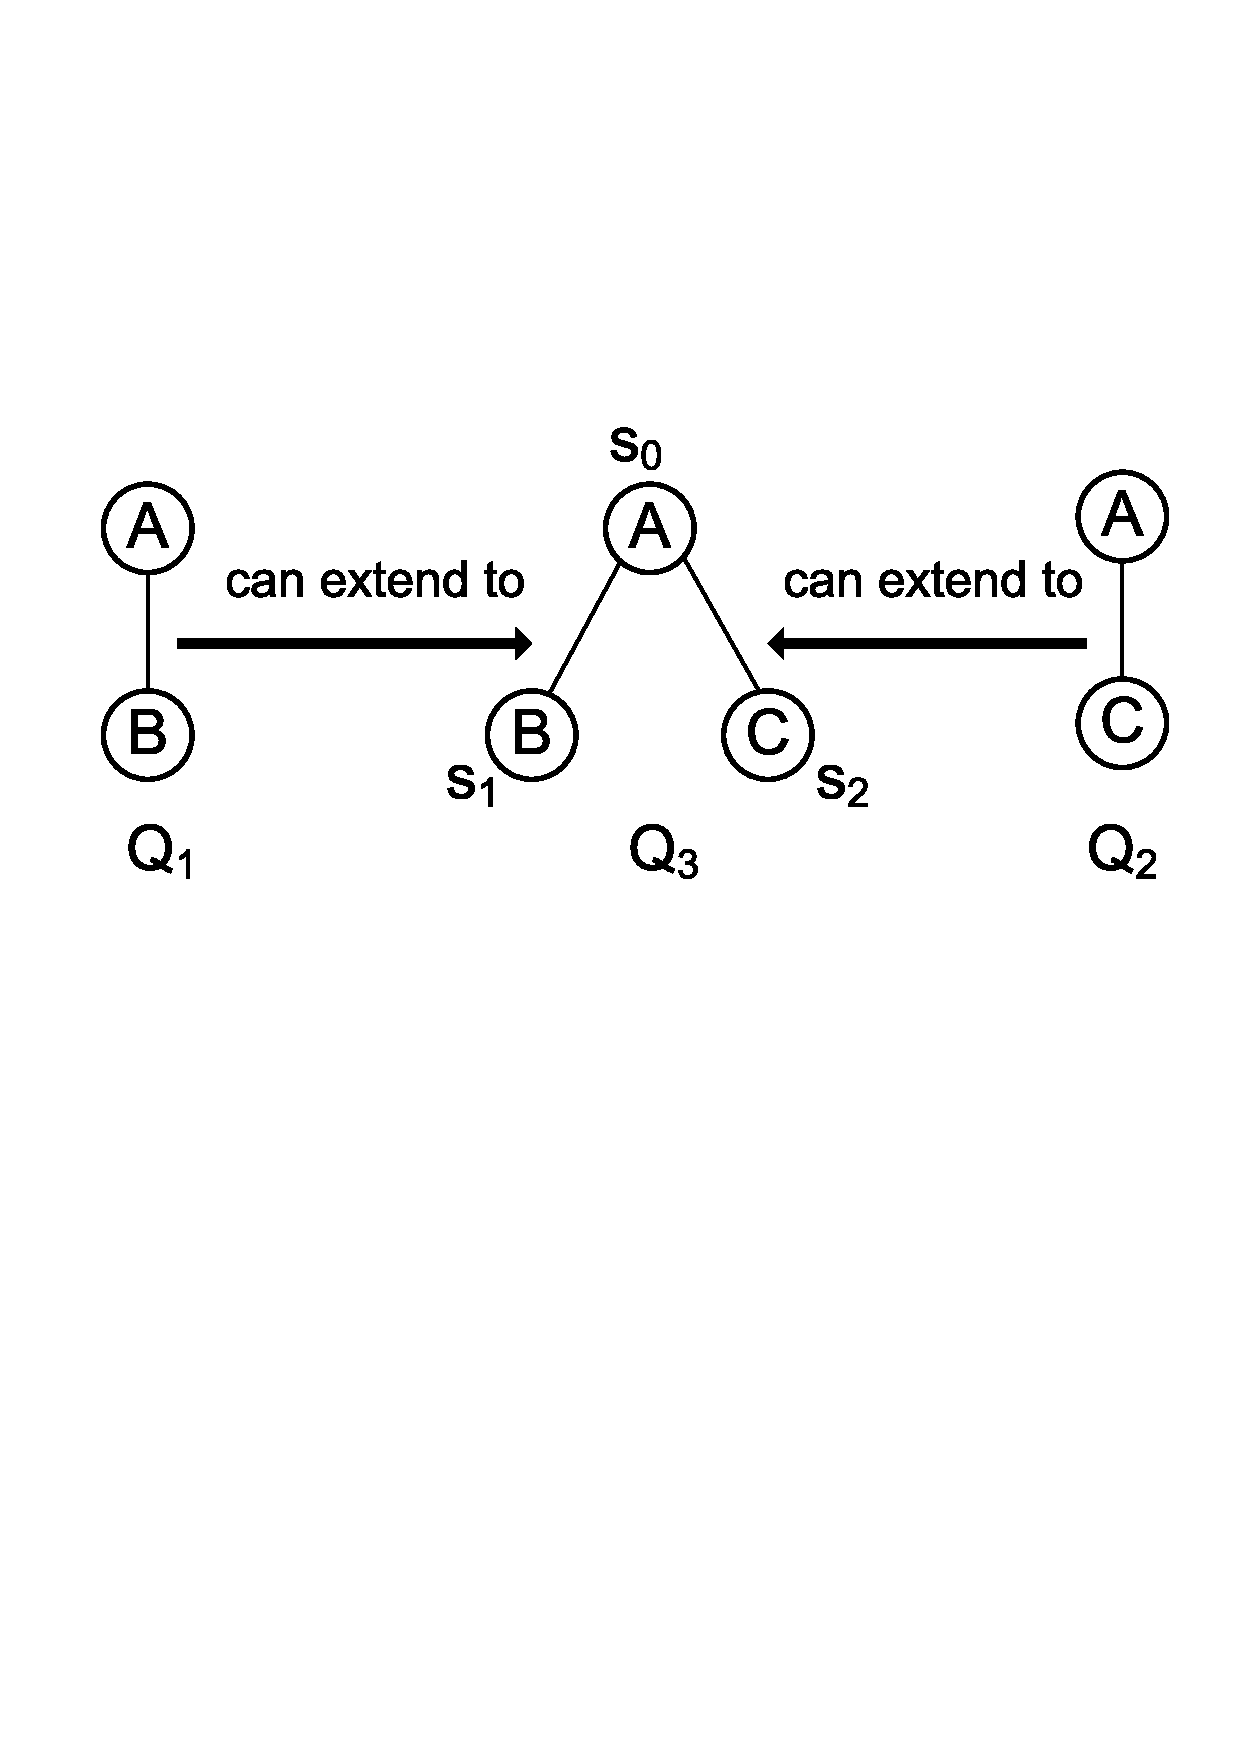
\includegraphics[scale=0.32]{images/avoiding}
	\vspace{-2mm}
	\caption{\scriptsize Subgraph $Q_1$ and $Q_2$ are the subgraphs of $Q_3$.}
	\label{fig:avoiding}
	\vspace{-6mm}
\end{figure}


\begin{exple}
	In Figure \ref{fig:avoiding}, suppose $Q_1$ extended to $Q_3$ and $Q_3$ knows that $Q_1$ is its subgraph. However, during {\sf Op($Q_3$)}, $Q_3$ must avoid the correlation $\tau(Q_3,Q_2,h)$ because $Q_2$ is also the subgraph of $Q_3$.
\end{exple}


Obviously, we can not use subgraph isomorphism to check this relationship of $Q_1,Q_2$ before the correlation calculation since it is too expensive. We use following approach to rapidly get the answer.
\par We first add one more rule to best-first-search, if $\sigma(Q_1)=\sigma(Q_2)$, $Q_1$ has higher priority to be operated if and only if:
\begin{align*} |V_{Q_1}|<|V_{Q_2}| \end{align*}
According to this rule, together with downward-closure, we could always
guarantee that $Q_1$ is extended before $Q_2$. \par For each subgraph $Q$, it
maintain a subgraph set $SubRec(Q)$, recording all of its subgraphs. Under our
assumption, $Q_1$ can extend to $Q_2$ so that $Q_2$ knows that $Q_1$ is the
subgraph of $Q_2$ and all the subgraphs of $Q_1$ are also the subgraphs of
$Q_2$. As a result, if $Q_1$ can extend to $Q_2$, then we operate
$SubRec(Q_2)=SubRec(Q_2)\cap Q_1\cap SubRec(Q_1)$. As {\sf Op($Q$)} is
occurring, if $Q_i\in SubRec(Q)$, we skip $\tau(Q,Q_i,h)$.

\section{Mining Algorithm}
\label{subsec:miningalgo}
The complete mining algorithm consists of an initialization step and the search
algorithm to compute top-\textit{k} pairs of correlated subgraph patterns. The
details of these procedures are described in the following subsections.
\subsection{Initialization}
\label{subsec:initialization}
Algorithm \ref{algo:initialization} specifies the step-by-step operations of the
initialization procedure.

\begin{algorithm}%[h!]
	\caption{\textsc{Initialization}}\label{algo:initialization}
	\dontprintsemicolon
	\nonl \textbf{Input:} Graph $G$, {\sf Min-Sup:} $min\_sup$, hop value: $h$\;
	\nonl \textbf{Output:} frequent edges set: $F\_edges$, proximate vertices
	index: $CorV$, modified data graph: $G$ \;
		% $F\_edges\leftarrow$ frequent edges from $E(G)$\;
		$F\_edges\leftarrow \{e\ |\ e \in E(G),\ \sigma(e) \geq min\_sup \}$\;
		\ForEach{\textup{$u \in V(G)$ such that $(u, u')$\ \in\ F\_edges\ \ }}
		{\textsc{BFS} from $u$ to all $v\in V(G)$, such that min distance
		$d(u,v)\le h$\; $CorV(u) \leftarrow$ set of all $v$ obtained above\;}
		$NF\_edge\leftarrow E(G)\setminus F\_edge$ \; Remove $NF\_edge$ from
		$E(G)$\; \Return {$F\_edges,\ CorV,\ G$}\;
	% \end{algorithmic}
\end{algorithm}

The algorithm begins with a brute-force search to obtain all frequent edges in
the data graph (line 2). Once the set of frequent edges (stored in variable
$F\_edges$) is computed, the algorithm executes a breadth-first search (BFS)
procedure (line 4) for every vertex $u$ that constitutes an edge in $F\_edges$
to obtain all vertices satisfying the hop constraint with respect to $u$. The
set of these vertices is stored in the $CorV$ dictionary mapped to $u$ (line 5).
Thus, the set of proximate vertices for every vertex constituting a frequent
edge is obtained and stored. Finally, the algorithm deletes the set of
infrequent edges from $G$ to obtain the modified data graph (lines 7-8).
Infrequent edges are removed since these have no bearing on the algorithm
hereafter and doing so accelerates the search procedure.
% The first step is get all the frequent edges of the data graph (line ). Then,
% for every vertex of the frequent edges, we use BFS to get all the other
% vertices which satisfies the hop-constraints with it (line ). We put the
% result in the distance index set after the BFS of one vertex and we get all
% the proximity vertex set of every vertex (line ). We use this union set as the
% original distance index. This index set contains everything of proximity
% vertices but contains nothing of proximity patterns. We will use this original
% set to create and maintain the index of proximity patterns, specified in
% Section \ref{subsec:search-steps}. Finally, we remove the infrequent edges
% from the data graph (line ) because they are useless after initialization and
% removing them could accelerate the search.

\subsection{Search Steps}
\label{subsec:search-steps}
Following the initialization, the search algorithm as specified in
Algorithm~\ref{algo:searchsteps} is executed.
\begin{algorithm}
	\dontprintsemicolon
	\caption{\textsc{Search}}\label{algo:searchsteps}
	\nonl \textbf{Input:} Graph $G$, {\sf Min-Sup:} $min\_sup$, frequent edges
	set: $F\_edges$, $CorV$, Generated patterns dictionary: $\mathbb{D}$ \;
	\nonl \textbf{Output:} $top\_k$ pairs of correlated subgraph patterns  \;
	Initialize {\sf Search Queue} with $F\_edges$ \; 
	\While{\textup{\textsc{CeasingCondition} is not satisfied}} 
	{
		subgraph $Q \leftarrow$ {\sf Search\
		Queue.Pop()}\; 
		Execute \textsc{Operate($Q$)}\; 
		$Ex(Q) \leftarrow $ \textsc{SubgraphEdgeExtensions($Q$)}\; 
		\ForEach{\textup{candidate edge} $e(u,v)\in Ex(Q)$} 
		{
			child $Q'\leftarrow Q$ extended with $e$\; 
			\uIf{$DFS\ Code(Q') \notin \mathbb{D}$}
			{
				$replica(Q') \leftarrow $ \textsc{GetReplica($Q', u, e, \dots$)}\;
				Compute $\sigma(Q')$ from $replica(Q')$\;
				\uIf {$\sigma(Q')\geq min\_sup$}
				{
					Push $Q'$ into \textsc{SearchQueue}\;
				}
				Record $DFS\ Code(Q')$ in $\mathbb{D}$\;
			}
			\Else
			{
				continue\;
			}
		}
	}
		\Return {$top\_k$ \textup{correlated pairs}}\;
	% \end{algorithmic}
\end{algorithm}

The algorithm begins with the initialization of a priority queue called
$Processing\_Queue$ (line 1) that stores subgraph patterns scheduled for
correlation computation with the property that a pattern with a higher
MNI-support is accorded a higher priority following the best-first search
strategy (Section~\ref{subsubsec:estimating}). $Processing\_Queue$ is
initialized with the set of frequent edges (queued in the order of decreasing
support values). During search, as long as the $ceasing\ condition$
(Section~\ref{subsubsec:ceasing}) remains unsatisfied, the subgraph pattern at
the front of $Processing\_Queue$ is selected for correlation computation and
extension. Correlation computation takes place in method {\sf Operate}
(Algorithm~\ref{algo:operate}) wherein the top-\textit{k} set can also be
updated. This is followed by the computation of all possible one edge extensions
in $Q$ in method {\sf Subgraph Edge Extensions} (line 5). For every candidate
extension in $Ex(Q)$, the DFS Code of the resulting child subgraph pattern $Q'$
is tested for presence in dictionary $\mathbb{D}$. A match in $\mathbb{D}$
indicates that $Q'$ has already been generated previously, so the algorithm
proceeds with the MNI-support computation only if there is no match (line 8).
MNI-support computation for $Q'$ requires the construction of its $replica$
structure, which the algorithm computes and stores through the invocation of
{\sf Get Replica} method described (line 9). Note that the $replica$ structure
for a child pattern not only establishes the MNI-support but also allows
correlation computation in method {\sf Operate}. If the child pattern's
MNI-support value exceeds the threshold $min\_sup$, it is pushed into
$Processing\_Queue$ (line 12) to be (possibly) processed in a later iteration of
the outer loop. $DFS\_Code(Q')$ is recorded in $\mathbb{D}$ (line 14).
% During the search step, if the ceasing condition in Section
% \ref{subsubsec:ceasing} is not satisfied, we select a subgraph $Q$ in
% $Leaf(T)$ according to the criteria in Section \ref{subsubsec:estimating}
% (line ). Then we process event {\sf Op($Q$)}, which calculate the correlation
% of $Q$ and put the result into {\sf Top-$k$} set if it satisfies the condition
% specified in Section \ref{sec:calculation} (line ), and extend $Q$ to a larger
% subgraph with one edge growth. If the new extension $Q'$ satisfies the MNI
% support, we process event {\sf Found($Q'$)} (line ). The loop goes on until
% the ceasing condition is satisfied.\\
% \begin{observation} \label{ob:frequency} If two subgraphs have higher support
% values individually, it is very likely that the pair will also have a higher
% correlation. \end{observation}

% \begin{observation} \label{ob:dfs} For highly (e.g., top-$k$) correlated
% subgraphs mining, generally a breadth-first or a best-first exploration of the
% search space is more efficient compared to a depth-first traversal of the
% search space. \end{observation}

% Obviously, by setting $k$ to infinity can we mine all the correlated
% subgraphs. However, on the contrary, it is hard to control the value of {\sf
% Min-sup} to get the result of a particular $k$ of {\sf Top-$k$} correlated
% subgraphs. That is to say, the {\sf Min-Sup} problem can be transfered from
% {\sf Top-$k$} problem. As a result, we concentrate on {\sf Top-$k$} problem in
% the following sections. 
\begin{figure}[t!]
	\centering
	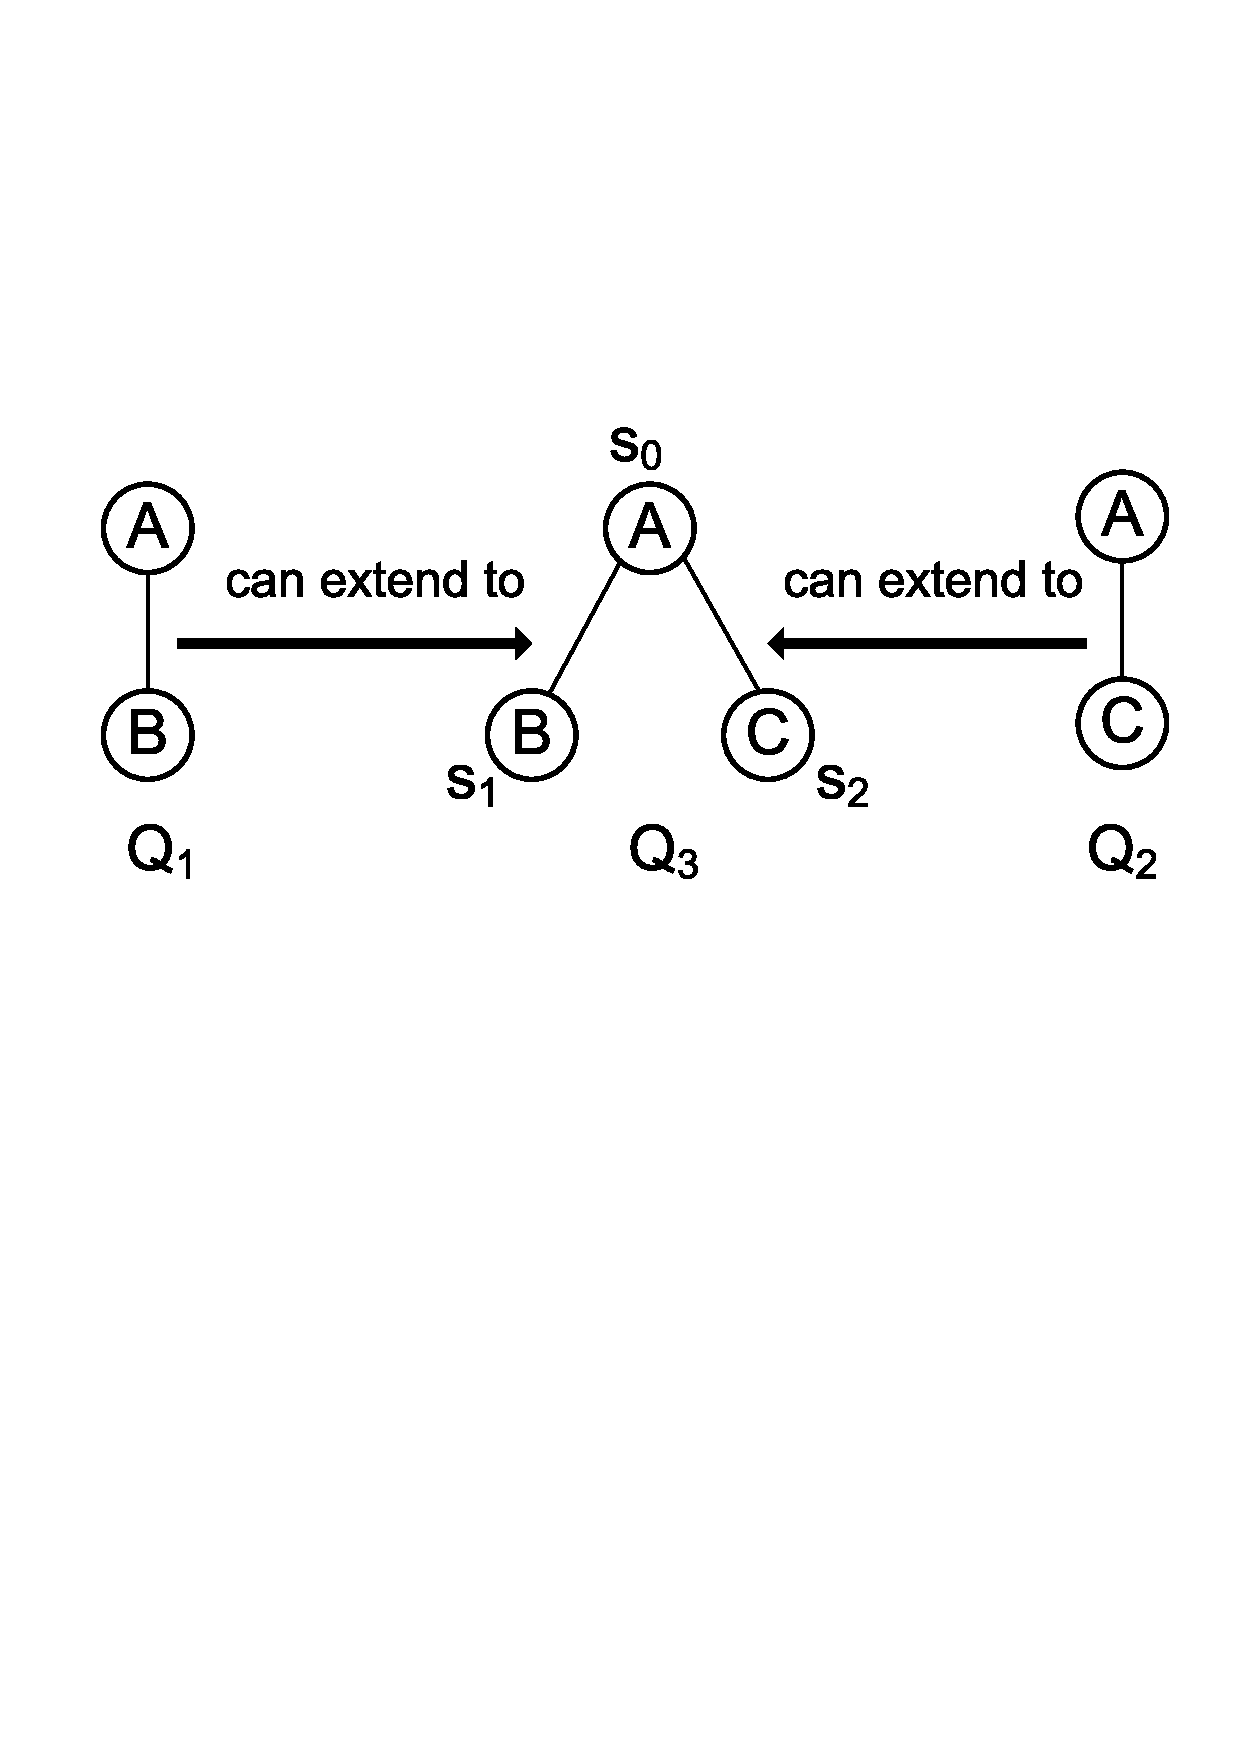
\includegraphics[scale=0.32]{images/avoiding}
	\vspace{-2mm}
	\caption{\scriptsize Subgraph $Q_1$ and $Q_2$ are the subgraphs of $Q_3$.}
	\label{fig:avoiding}
	\vspace{-6mm}
\end{figure}


% \begin{figure}[t!]
% 	\vspace{2mm}
% 	\centering
% 	\subfigure[{\scriptsize Hello World }]
% 	{
% 		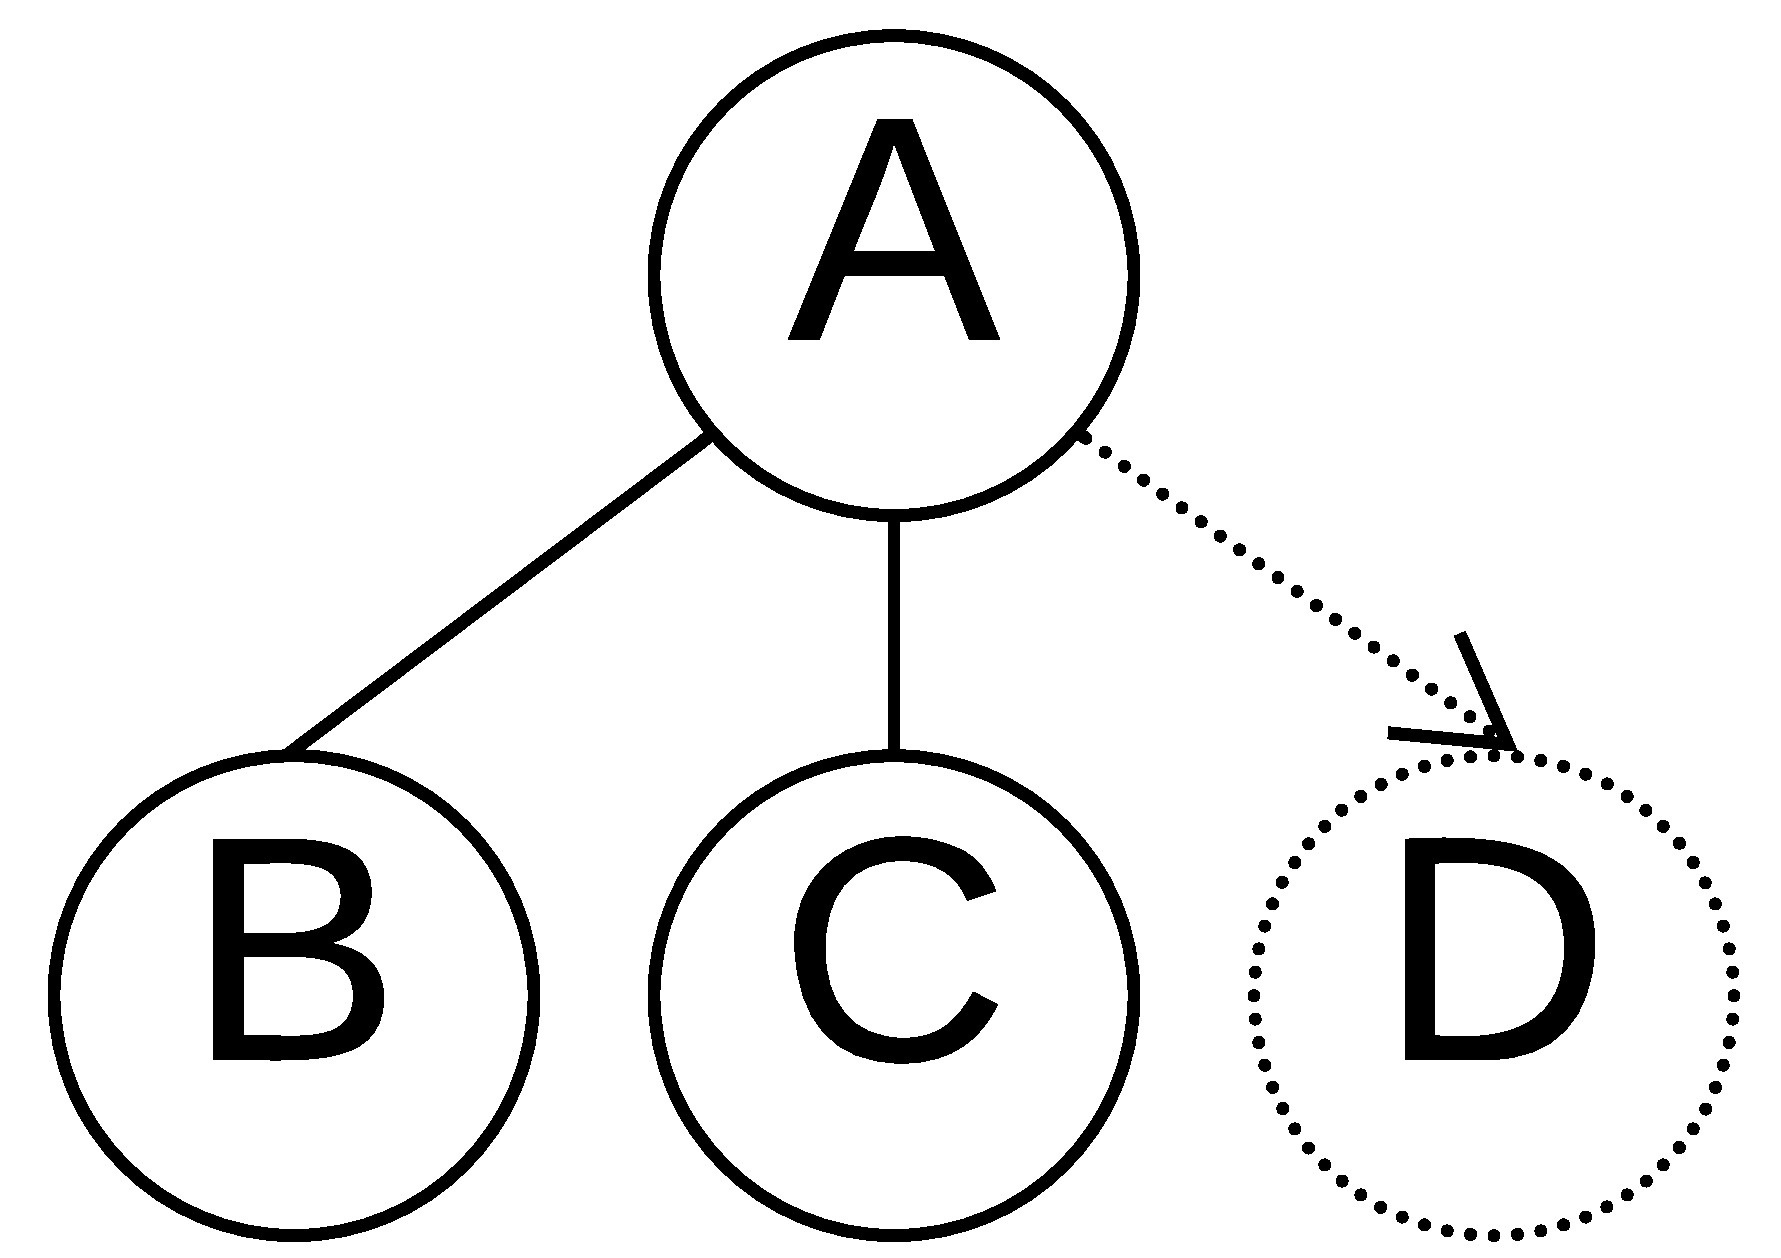
\includegraphics[scale=0.06]{img_ex/temp1.pdf}
% 		\label{subfig:exp_temp1}
% 	}
% 	\vspace{-2mm}
% 	\caption{\scriptsize Get Replica}
% 	\label{fig:exp_temp1}
% 	\vspace{-2mm}
% \end{figure}

\begin{figure}[t!]
	\centering
	\subfigure[{\scriptsize Subfig1}]	
	{
		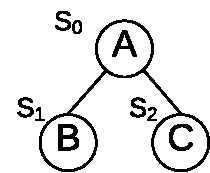
\includegraphics[scale=0.07]{img_ex/Exact-Q.pdf}
		\label {subfig:exact_Q}
	}
	\subfigure[{\scriptsize Subfig2}]
	{
		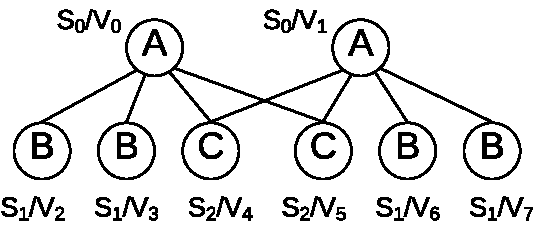
\includegraphics[scale=0.07]{img_ex/Exact-rep(Q).pdf}
		\label {subfig:exact_repQ}
	}
	\vspace{-2mm}
	\caption{\scriptsize GetReplica}
	\label{fig:avoiding}
	\vspace{-6mm}
\end{figure}

